% enable this to activate the version for PRINT
% disable this to make the pdf symmetric and without white pages
% => asymmetric alternating left/right margins
%%\newcommand*{\printversion}{}%

%% | ---------------- document meta information --------------- |

\newcommand{\Author}{Michal Werner}
\newcommand{\Department}{Department of Computer Science}
\newcommand{\Supervisor}{Ing. Tomáš Báča, Ph.D.}
\newcommand{\SupervisorSpecialist}{Ing. My Specialist, Ph.D.}
\newcommand{\Programme}{Open Informatics}
\newcommand{\Field}{Artificial Intelligence}
\newcommand{\Title}{Localization of sources of ionizing radiation using a group of unmanned aerial vehicles}
\newcommand{\Keywords}{Unmanned Aerial Vehicles, Automatic Control}
\newcommand{\KlicovaSlova}{Bezpilotní Prostředky, Automatické Řízení}
\newcommand{\Year}{2021}
\newcommand{\Month}{January}
\newcommand{\Date}{\Month~\Year}
\newcommand{\Location}{Prague}
\newcommand{\mycomment}[1]{}
%% | ---------------------- configuration --------------------- |

% most of the configuration stuff happens here
\input{src/document_setup.tex}

%% | ---------------------- the contents ---------------------- |

\begin{document}

\pagenumbering{roman}

%% --------------------------------------------------------------
%% |                         Title page                         |
%% --------------------------------------------------------------

\input{src/title}

% set up the page style for the "intro" pages
\pagestyle{plain}

%% --------------------------------------------------------------
%% |                       Acknowledgments                      |
%% --------------------------------------------------------------

\conditionalClearPage

%!TEX root = ../main.tex

\section*{Acknowledgments}
%First of all, I would like to express my gratitude to my supervisor for all his support, guidance and valuable advices during this project.
%Secondly, I want to express my appreciation to my classmates and colleagues for the all the well spend study time, many and many created memes and mutual support during our challenging study period.
%I am also thankful to my family for all the support they provided my during my studies. %, that  forget to thank my family for all their support throughout my studies.
%Finally, I would like to express my appreciation to everyone who ensures that the research topic of this work would never be needed in practice, and that the radiation situation in Czechia, in Ukraine and everywhere else) would "remain normal."
First of all, I would like to express my gratitude to my supervisor for all his support, guidance, and valuable advice during this project.
Secondly, I want to express my appreciation to my classmates and colleagues for the time we spent studying together, the countless memes we created, and the mutual support we provided each other during our challenging study period.
I am also thankful to my family for their unwavering support throughout my studies.
Finally, I would like to express my appreciation to everyone who ensures that the research topic of this work would never be needed in practice and that the radiation situation in Czechia, Ukraine, and everywhere else in the world remains normal.

\vspace{2.5cm}








\section*{Poděkování}
Nejprve bych rád vyjádřil svou vděčnost svému vedoucímu za veškerou podporu, vedení a cenné rady během tohoto projektu. 
Zadruhé bych chtěl vyjádřit své díky svým spolužákům a kolegům za čas, který jsme spolu strávili studiem, nespočet vytvořených memů a vzájemnou podporu během našeho náročného studijního období. 
Jsem také vděčný své rodině za jejich neochvějnou podporu během celého mých studií. 
Nakonec bych chtěl vyjádřit své uznání všem, kdo se starají o to, aby výzkumné téma této práce nebylo nikdy potřeba v praxi a aby radiační situace v České republice, na Ukrajině a všude jinde zůstala normální.

%Chtwl bych poděkovat vedoucímu mé práce za veškerou podporu, cenné rady a předané zkušenosti.
%Zadruhé děkuji svým spolužákům a kolegů za všechen ten čas společně strávený studiem, mnoho a mnoho vytvořených memů a vzájemnou podporu během náročných studií.
%Děkuji také své rodině za veškerou podporu během celé doby studia.
%Nakonec bych chtěl poděkovat všem, kteří se starají o to, aby výzkumné téma této práce nebylo nikdy potřeba v praxi a radiační situace zůstávala normální. 


%% --------------------------------------------------------------
%% |                         Assignment                         |
%% --------------------------------------------------------------

\conditionalClearPage

\includepdf{src/assignment.pdf}

%% --------------------------------------------------------------
%% |                          Abstracts                         |
%% --------------------------------------------------------------

\conditionalClearPage

%!TEX root = ../main.tex

\begin{changemargin}{0.8cm}{0.8cm}

~\vfill{}

\section*{Abstract}
\vskip 0.5em

This thesis presents a method for localizing multiple sources of ionizing radiation using a group of \acp{UAV}. 
These \acp{UAV} are equipped with miniature single-detector Compton camera radiation sensors, enabling them to estimate the directions towards high-energy gamma radiation sources.
  The proposed radiation mapping method (utilizing a \ac{MLE} principle) fuses the measurements from the Compton camera sensors to accurately estimate the positions of radioactive sources during the flight.
The properties of the used detector are approximated using Monte Carlo simulation techniques.
The estimation method is combined with an active search strategy that coordinates future action of the drones in order to improve the quality of estimate of sources position and minimize search time.
%In addition, an active search strategy is incorporated into the system, coordinating the future actions of the drones. 
%This strategy aims to improve the quality of the estimated source positions and minimize the search time by efficiently exploring the designated area of interest.
The proposed solution is evaluated on recorded real world data and in realistic simulator.





  \mycomment{
%The study of autonomous \acp{UAV} has become a prominent sub-field of mobile robotics.

This thesis presents a method for localization of multiple sources of ionizing radiation using a group of autonomous \acp{UAV} 
that are equipped with a miniature single-detector Compton camera radiation sensor capable of estimating directions towards a source of high-energy gamma radiation.
The proposed radiation mapping method (based on a \ac{MLE} principle) fuses the measurements from the Compton camera sensors and estimates the positions of radioactive sources during the flight.
Properties of the detector are approximated using Monte Carlo simulation.
The estimation method is combined with an active search strategy that coordinates future action of the drones in order to improve the quality of estimate of sources position and minimize search time.
The solution is evaluated on recorded real world data and in realistic simulator.
%The proposed estimation method based on maximum likelihood principle fuses the Compton camera measurements and estimates the positions of radioactive sources during the flight.
%The MiniPIX TPX3 Compton camera is can electronvolt
%The proposed solution utilizes a data fusion method based on \ac{MLEM} algorithm, which combines measurements from multiple \acp{UAV} and estimates the positions of radioactive sources during the flight.
%The fusion method 

%  for fusing the measurements
%and estimating the radiation source position during the flight.
}
\vskip 1em

{\bf Keywords} \Keywords

\vskip 2.5cm

\end{changemargin}


\conditionalClearPage

%!TEX root = ../main.tex

\begin{changemargin}{0.8cm}{0.8cm}

~\vfill{}

\section*{Abstrakt}
\vskip 0.5em

\sloppy

Tato práce představuje metodu lokalizace více zdrojů ionizující radiace pomocí bezpilotních prostředků (dronů).
Tyto drony jsou vybaveny miniaturním detektorem fungujícím na pripcipu jednovrstvé Comptonovy kamery, který umožňuje odhadovat směry k zdrojům vysokoenergetického gama záření.
Navržená metoda pro mapování radiace (založená na principu maximální věrohodnosti) kombinuje měření z Comptonových kamer a za letu odhaduje pozice radioaktivních zdrojů.
Vlastnosti použitého senzoru jsou odhadnuty pomocí Monte Carlo simulace.
Metoda odhadu pozice zdrojů je je kombinována s aktivní prohledávací strategií, která koordinuje pohyb bezpilotních helikoptér za účelem zlepšení kvality odhadu pozice zdrojů radiace a minimalizace času potřebnému k jejich nalezení. 
Navžené řešení je otestováno na dříve naměřených datech ze skutečných senzorů a pomocí realistického simulátoru.

\vskip 1em

{\bf Klíčová slova} \KlicovaSlova

\vskip 2.5cm

\end{changemargin}


%% --------------------------------------------------------------
%% |                        Abbreviations                       |
%% --------------------------------------------------------------

\conditionalClearPage

\begin{changemargin}{0.8cm}{0.8cm}

~\vfill{}

\section*{Abbreviations}

% this will print only the used abbreviations
%!TEX root = ../main.tex

\begin{acronym}
  \acro{API}[API]{Application Programming Interface}
  \acro{CTU}[CTU]{Czech Technical University}
  \acro{DOF}[DOF]{degree-of-freedom}
  \acro{FOV}[FOV]{Field of View}
  \acro{GNSS}[GNSS]{Global Navigation Satellite System}
  \acro{GPS}[GPS]{Global Positioning System}
  \acro{IMU}[IMU]{Inertial Measurement Unit}
  \acro{MLE}[MLE]{Maximum likelihood estimation}  
  \acro{LKF}[LKF]{Linear Kalman Filter}
  \acro{CS}[CS]{Compton scattering}
  
  \acro{PE}[PE]{Photoelectric effect}
  \acro{PET}[PET]{Positron emission tomography}
  \acro{SPECT}[SPECT]{Single Photon Emission Computed Tomography}
  \acro{FDNPP}[FDNPP]{Fukushima Daiichi Nuclear Power Plant}
  \acro{LM-MLEM}[LM-MLEM]{List Mode-Maximum Likelihood Expectation Maximization}

  \acro{TSP}[TSP]{Travelling salesman problem}
  \acro{MAV}[MAV]{Micro Aerial Vehicle}
  \acro{MPC}[MPC]{Model Predictive Control}
  \acro{MRS}[MRS]{Multi-robot Systems Group}
  \acro{ROS}[ROS]{Robot Operating System}
  \acro{SLAM}[SLAM]{Simultaneous Localization And Mapping}
  \acro{UAV}[UAV]{Unmanned Aerial Vehicle}
  \acro{UGV}[UGV]{Unmanned Ground Vehicle}
\end{acronym}


\vskip 2.5cm

\end{changemargin}

\conditionalClearPage

%% --------------------------------------------------------------
%% |                      Table of contents                     |
%% --------------------------------------------------------------

\tableofcontents

\conditionalClearPage

% set up the full page style with normal page numbering
\pagestyle{full}
\pagenumbering{arabic}

%% --------------------------------------------------------------
%% |                        introduction                        |
%% --------------------------------------------------------------
\acresetall
%!TEX root = ../main.tex
\chapter{Introduction\label{chap:introduction}}
The field of mobile robotics has undergone significant progress in the past decades.
Robots are nowadays capable of performing a wide variety of tasks. 
Such systems can be more efficient than human workers and can replace them in environments that are dangerous for human beings.
One possible application for autonomous robots is the mapping and monitoring of ionizing radiation. 
Radioactive materials are part of our world, and there are several situations when such a need might occur, for example, a disaster in a nuclear power plant or misuse of materials for radiotherapy in medicine. 
To ensure public safety, we need a method for fast and efficient localization of radioactive sources without the presence of human workers.
A \ac{UAV} (frequently referred as a drone) equipped with appropriate sensors is a promising solution to this problem.
A group of highly mobile \ac{UAV}s can quickly and autonomously explore large areas and perform measurements needed for precise localization of radioactive sources.

Sensing ionizing radiation is possible thanks to the variety of sensors, one of which is called the Compton camera.
The Compton camera utilizes the Compton scattering effect, which was discovered by Arthur Compton in 1923 \cite{compton}.
During the Compton scattering, an ionizing photon interacts with an electron and scatters (the photon's direction is changed while part of the photon's energy is transferred to the electron).
This principle allows the Compton camera to not only detect the presence of ionizing particles (as common in intensity-based sensors, such as widely known dosimeters), but also reconstruct a set of possible directions from where the photon arrived to the sensor.
Thanks to innovations in the field of sensory equipment, Compton camera \ac{pix} became small and lightweight enough to be carried by a small \ac{UAV} onboard.


\begin{figure}[!h]
    \centering
  \includegraphics[width=0.6\textwidth]{./fig/photos/uav.jpg}
    \caption{A small T650 multi-rotor UAV equipped with the \ac{pix} sensor. Source: \cite{baca2021gamma}.}
    \label{fig:uavvv}
\end{figure}

This thesis aims to present a method that performs the fusion of sensory data from multiple \ac{UAV}s (equipped with Compton camera sensor) in order to localize multiple sources of ionizing radiation.
The estimation method is based on the \ac{MLEM} algorithm that estimates distribution of sources of ionizing radiation while maximizing likelihood of measured data.
The localization of radioactive sources is performed online during the flight.
Thanks to the online estimation, the group of \ac{UAV}s autonomously adapts its actions accordingly  in order to increase the precision of the estimate and minimize the search time.
The presented data fusion method, as well as the high-level search strategy, are tested in simulations and on prerecorded data from real-world experiments.

\section{Related work}
The remote sensing of ionizing radiation is a very broad topic involving many disciplines, such as medicine, astronomy, industry, public safety or robotics.
The overview presented in \cite{radiation_detection_systems_overview} shows various mobile radiation detection systems, sensors and reconstruction methods that were presented in the past decade.
The focus of this thesis is on remote sensing using unmanned vehicles.
Several works describing radiation mapping using robots appeared after 2011 when the biggest radioactive accident in past decades happened in Japan.
The strong earthquake and following tsunami wave caused several leakages of radioactive substances from \ac{FDNPP}.
The contaminated area of the powerplant was explored by \ac{UGV}s (\cite{fuku2012,fuku_compton}) as well as \ac{UAV}s equipped with different radioactivity sensors (\cite{sanada2015, towler2012, Jiang2015, Mochizuki_2017, sato_drone_compton_camera_2018}).

%\subsubsection{Intensity-based methods}
Sensors used for remote monitoring of ionizing radiation can be generally classified into two groups: intensity-based and direction-based.
Intensity-based detectors measure only the number of particles recorded in the sensor (particle flux at the sensor's position).
The distribution of radioactive material is then estimated thanks to measurements acquired at different positions.
A group of \ac{UGV}s remotely sensing contaminated indoor area is presented in \cite{fuku2012}.
Radiation mapping of a large-scale area around the \ac{FDNPP} powerplant using an unmanned helicopter equipped with large scintillation intensity-based detectors is shown in \cite{sanada2015} and \cite{towler2012}.
Multi-rotor \ac{UAV}s have been used for remote sensing in \cite{nine_drone_fukushima, ten_remote_sensing_with_uderstanding_uav_ugv} and \cite{eleven_remote_sensing_non_japan}.
In most of the presented experiments, the \ac{UAV}s were following predefined trajectories.
The radiation mapping was done offline after the flight.

A recent paper \cite{mascarich2022} presents a method for radiation mapping in the indoor environment.
The method is based on estimating the gradient of radiation from multiple intensity-based measurements.
The onboard sensors can not only localize the sources of radioactivity but also estimate the energetic spectrum of measured particles and decide which radioactive material is detected.
Moreover, the authors have presented an active search path planning method that plans the movement of the drone in order to improve the quality of measurements and shorten the search time.

Work presented in \cite{stibinger2020} shows a method for radioactivity mapping using intensity-based dosimetric measurements acquired by the same sensor as in this thesis.
Each drone measured intensities in multiple directions while hovering at the actual position.
The direction with the highest intensity was chosen as a direction vector towards the source.
These directions vectors acquired at different positions were fused using \ac{LKF}.
However, this method is not designed for the localization of multiple sources of radiation.

This thesis focuses on the direction-based sensor --- the Compton camera.
Radiation mapping around \ac{FDNPP} using an \ac{UAV} equipped with a Compton camera is presented in \cite{Jiang2015}, \cite{Mochizuki_2017}, \cite{sato_drone_compton_camera_2018}.
In all cases, the platforms were hovering for a certain time above the predefined positions and the radiation images were reconstructed offline after the flight.
Work presented in \cite{fuku_compton} shows a radioactive hotspot localization inside the \ac{FDNPP} by one \ac{UGV} equipped with a Compton camera.
However, this work focused only on 2D image reconstruction, and the robot was moving only in one direction during the experiment.
A 3D localization of a single radioactive source (using an \ac{UGV} equipped with a Compton camera) is presented in \cite{3D_compton_mobile_robot_2017}.
The authors combine \ac{SLAM} method (estimating the 3D map of the environment) with Compton camera measurements. % in order to reconstruct a 3D position of a radioactive source.
The \ac{UGV} stops at predefined positions for $\SI{5}{\minute}$ and collects around $4000$ Compton measurements during the presented simulated experiment.
The reconstruction method is based on the iterative \ac{MLEM} algorithm, the same as in this work.
However, the authors of the paper do not specify the details of the proposed \ac{MLEM} reconstruction method (the system matrix is not further described).

The \ac{MLEM} reconstruction method was originally developed for nuclear medicine imaging, as described in one of the following chapters.
Except few applications in robotic ionizing radiation sensing (\cite{fuku_compton}, \cite{3D_compton_mobile_robot_2017}), authors of \cite{handheld_mlem_reconstruction}
present a handheld device for the localization of radioactive sources. 
The presented device is composed of an omnidirectional imaging system (capable of acquiring Compton measurements) as well as a \ac{LiDAR} sensor.
%The reconstruction method is also based on \ac{MLEM} algorithm.
The \ac{MLEM} estimate is combined with a 3D map of the environment, created from \ac{LiDAR} measurements using a \ac{SLAM} method.
The device weighting $\SI{6.3}{\kilogram}$ is capable of online estimation of radioactive sources.
Another handheld device with an online reconstruction method for Compton camera measurements is presented in \cite{handheld_visual}.
Authors there combine visual data with radiation estimate computed using \ac{MLEM} method (without evaluating the sensitivity of detection).

In general, one of the key limiting factors is the size of the sensor.
There is a tradeoff between the detector's size and the detector's sensitivity.
The bigger the sensor is, the more ionizing particles can measure (given the nature of the radiation).
On the other hand, heavy and bulky sensors must be carried by \ac{UGV}s or \ac{UAV}s with a sufficient load capacity that reduces their operability. 
Ground robots can't compete with aerial platforms in the speed of exploration and flexibility. 
Large aerial platforms (unmanned helicopters) can't fly close to the obstacle due to safety reasons.
This motivates the use of small \ac{UAV}s equipped with small direction-based sensors.
The limited sensor's sensitivity can be compensated by the use of multiple \ac{UAV}s cooperating together on the given task.
Moreover, small \ac{UAV}s can fly closer to obstacles (acquire more measurements) and use the full potential of small agile aerial platforms (acquire measurements from different positions simultaneously and therefore find sources of radiation in a shorter time).
This could be achieved thanks to the lightweight \ac{pix} \cite{baca2019timepix} sensor, which is further described in the next section.

This thesis builds on the work of the MRS group (Faculty of Electrical Engineering, CTU in Prague) that explored the possibilities of \ac{pix} sensor deployment onboard a small \ac{UAV}s. 
Paper \cite{baca2021gamma} presents a multi-robotic approach to an autonomous localization of a compact gamma radiation source. 
All unmanned aerial vehicles are equipped with a \ac{pix} sensor same as in our work), which is capable of measuring gamma particles and reconstructing Compton events. 
The reconstructed Compton cones are used for localization in the following way.
In the first phase of autonomous exploration, the \ac{UAV}s are exploring the area to measure the first Compton cones. 
After the first eight cones are reconstructed, their intersection is computed using optimization methods (quadratic programming). 
This initial estimate is then incrementally updated using new measurements. 
The current estimate is always orthogonally projected to the newly measured cone. 
These measurements are fused using \ac{LKF}. 
The \ac{UAV}s are controlled in a way that they encircle the current estimate in order to measure more cones and update the \ac{LKF} estimate.
Using this approach, the group of drones is capable of localizing a single compact source of ionizing radiation. 
The source can be static or dynamic. 
However, this iterative method cannot localize multiple sources of radiation.
Once the drones detect one source of radioactive particles, they start encircling the current estimate and cannot find other sources in the area.

To the author's best knowledge, there are no related works that solve the task of online autonomous multi-robot mapping of multiple sources of ionizing radiation with the use of a lightweight Compton camera sensor (e.g. \ac{pix}).

\section{Contributions}
The main contribution of this thesis is a novel approach to the localization of multiple compact radioactive sources based on Compton imaging.
The main purpose of this thesis is to improve the solution presented in \cite{baca2021gamma} in the following ways: 
firstly, introduce a new method that could localize multiple sources of ionizing radiation based on the measured Compton cones and, 
secondly, 
design high-level planning approach that would control a group of \ac{UAV}s in order to autonomously explore the whole area and maximize the chance that all sources of ionizing radiation would be detected while estimating their relative emission activity.

\section{Thesis organization}
The chapter \ref{chap:preliminaries} describes basic properties of ionizing radiation and its interactions with matter, the working principle of the Compton camera and \ac{pix} sensor.
The theoretical background of \ac{MLEM} estimation method is provided in the chapter \ref{chap:mlem_theory}.
The chapter \ref{chap:methods_estimation} presents the proposed radiation mapping method for a group of \ac{UAV}s equipped with a \ac{pix} Compton camera sensor.
The chapter \ref{chap:methods_robotics} describes the search strategy that controls the \ac{UAV}s in order to improve the precision of radiation mapping, acquire more measurements and explore the area of interest. 
Finally, the proposed methods were tested both in simulation and on real-world data. 
The results are presented in the chapter \ref{chap:results}.


\mycomment{\section{TRASH}% %%{

% %%{
%Reconstruction methods for Compton imaging were originally developed in the field of nuclear medicine.
%An overview of such methods is provided in one of the following chapters.
%\ac{MLEM} reconstruction methods are also used for radiation mapping.

%Multiple experiments with both  platforms were conducted in the neighbourhood of the \ac{FDNPP}.
%In 
%\cite{Jiang2015} presented an unmanned aerial platform equipped with a Compton camera. 
%In all these works, relatively large \ac{UAV} was following a predefined trajectory, and the computations were conducted offline.

%More recent works, such as TODO...
% %%}

% %%{
%compton ground robot

\subsubsection{Compton imaging in robotics}

Work presented in \cite{fuku_compton} showed a radioactive hotspot localization inside the \ac{FDNPP} by one \ac{UGV} equipped with Compton camera.
However, this work focused only on 2D image reconstruction, and the robot was moving only in one direction during the experiment.
3D localization of a radioactive source (using an \ac{UGV} equipped with a Compton camera) is presented in \cite{3D_compton_mobile_robot_2017}.
The authors combine \ac{SLAM} method with Compton measurements. % in order to reconstruct a 3D position of a radioactive source.
The \ac{UGV} stops at predefined positions for $\SI{5}{\minute}$ and collects around $4000$ Compton measurements during the presented simulated experiment.
The reconstruction method is based on iterative \ac{MLEM} algorithm, same as in this work.
However, authors of the paper do not specify the details of the proposed \ac{MLEM} reconstruction method (the system matrix is not further described).

%Paper \cite{china_robot_compton_moving_source} presents a  

Speaking of aerial platforms, a radiation mapping around \ac{FDNPP} using an \ac{UAV} equipped with a Compton camera is presented in \cite{Jiang2015}, \cite{Mochizuki_2017}, \cite{sato_drone_compton_camera_2018}.
In all cases, the platforms were hovering for certain time above the predefined positions and the radiation images were reconstructed offline after the flight.


%$\SI{90}{\kilogram}$ 






%\section{SOTA}



%The reconstruction methods based on \ac{MLEM} approach are presented in \cite{3D_compton_mobile_robot_2017
% %%}
%compton handheld

%Another application of \ac{MLEM} reconstruction technique is shown  

%\cite{nine_drone_fukushima}
%\cite{ten_remote_sensing_with_uderstanding_uav_ugv} %outside japan
%\cite{eleven_remote_sensing_non_japan}
%timepix sensor



%ideas%%{
%The advantage of \ac{UGV} is that they can carry heavier sensory equipment compared to \ac{UAV}s.
%On the other hand, the operability of ground robots is limited compared to aerial robots.
%The size of the detector is the main limiting factor.
%The smaller and lighter the detector (the aerial platform carrying it) is, the closer it can fly to the obstacles,
%on the other hand, the lower is the sensor's sensitivity (less particles intersects with the matter of the detector).

%Such method is used in \cite{sanada2015, towler2012}, where the unmanned helicopters were equipped with large scintillators.%%}




}% %%}
\mycomment{
\section{Mathematical notation}% %%{

It is a good practice to define basic mathematical notation in the introduction.
See \reftab{tab:mathematical_notation} for an example.

\begin{table*}[!h]
  \scriptsize
  \centering
  \noindent\rule{\textwidth}{0.5pt}
  \begin{tabular}{lll}
    $\mathbf{J}$  & set of discretized map positions indexed with $j$, $j \in (1, \dots, J)$ \\
    $\mathbf{I}$  & set of Compton measurements $i$, $i \in (1, \dots, I)$ \\
    $\mathbf{S}$   &  sensitivity vector with elements $s_{j}$, $\mathbf{S} \in \mathbb{R}^{J}$ \\
    $\mathbf{T}$   & system matrix with elements $t_{ij}$, $\mathbf{T} \in \mathbb{R}^{I \times J}$ \\
    $v$            & sampled drone position (composed of 3D position and orientation) \\
    $\beta$       & Compton angle
    %$\mathbf{U}$, $\bm{\alpha}$ & vector, pseudo-vector, or tuple\\
    %$\mathbf{\hat{x}}$, $\bm{\hat{\omega}}$& unit vector or unit pseudo-vector\\
    %$\mathbf{\hat{e}}_1, \mathbf{\hat{e}}_2, \mathbf{\hat{e}}_3$ & elements of the \emph{standard basis} \\
    %$\mathbf{X}, \bm{\Omega}$ & matrix \\
    %$\mathbf{I}$ & identity matrix \\
    %$x = \mathbf{a}^\intercal\mathbf{b}$ & inner product of $\mathbf{a}$, $\mathbf{b}$ $\in \mathbb{R}^3$\\
    %$\mathbf{x} = \mathbf{a}\times\mathbf{b}$ & cross product of $\mathbf{a}$, $\mathbf{b}$ $\in \mathbb{R}^3$\\
    %$\mathbf{x} = \mathbf{a}\circ\mathbf{b}$ & element-wise product of $\mathbf{a}$, $\mathbf{b}$ $\in \mathbb{R}^3$ \\
    %$\mathbf{x}_{(n)}$ = $\mathbf{x}^\intercal\mathbf{\hat{e}}_n$ & $\mathrm{n}^{\mathrm{th}}$ vector element (row), $\mathbf{x}, \mathbf{e} \in \mathbb{R}^3$\\
    %$\mathbf{X}_{(a,b)}$ & matrix element, (row, column)\\
    %$x_{d}$ & $x_d$ is \emph{desired}, a reference\\
    %$\dot{x}, \ddot{x}, \dot{\ddot{x}}$, $\ddot{\ddot{x}}$ & ${1^{\mathrm{st}}}$, ${2^{\mathrm{nd}}}$, ${3^{\mathrm{rd}}}$, and ${4^{\mathrm{th}}}$ time derivative of $x$\\
    %$x_{[n]}$ & $x$ at the sample $n$ \\
    %$\mathbf{A}, \mathbf{B}, \mathbf{x}$ & LTI system matrix, input matrix and input vector\\
    %\emph{SO(3)} & 3D special orthogonal group of rotations\\
    %\emph{SE(3)} & \emph{SO(3)}~$\times~\mathbb{R}^3$, special Euclidean group\\
  \end{tabular}
  \noindent\rule{\textwidth}{0.5pt}
  \caption{Mathematical notation, nomenclature and notable symbols.}
  \label{tab:mathematical_notation}
\end{table*}% %%}
}


%!TEX root = ../main.tex

\chapter{Preliminaries\label{chap:preliminaries}}

\section{Radioactivity}
Radioactivity is a natural phenomenon in which unstable atomic nuclei undergo spontaneous decay, emitting radiation in the form of particles or electromagnetic waves. 
This process occurs in certain types of atoms, known as radioactive isotopes or radionuclides. 
A radioactive atom attempts to reach stability by releasing energy in form of ionizing radiation.
Ionizing radiation refers to any form of radiation with enough energy to remove tightly bound electrons from the orbit of an atom.
Among others, radioactive decay releases three main types of ionizing radiation: alpha particles, beta particles, and gamma rays. 


\section{Properties of ionizing radiation}
\subsection{Activity}% %%{
"Activity" is one of the terms used to quantify and describe properties of radioactive sources.
It is defined as number of radioactive decays per second.
The unit of activity is called Becquerel ($\si{\becquerel}$) and belongs to SI\footnote{International System of units} units.
In other words, if a radioactive source has activity one Becquerel, it means that one unstable nucleous decays per second (on average, since the decay is a stochastic process).
It is important to note that the Becquerel only measures the rate of decay and does not take into account the type or energy of the radiation involved.% %%}

  \subsection{Inverse square law}% %%{
The inverse square law is a fundamental principle that applies to diverse physical phenomena including radiation.
It describes how the intensity of radiation decreases with increasing distance from the source.
The intensity of radiation is inversely proportional to the square distance from the source:
\begin{equation}
  intensity \approx \frac{1}{distance^2}.
\end{equation}
For example doubling the distance to the source means that the intensity decreases to $\frac{1}{4}$.
As illustrated in figure \ref{fig:islaw}, this principle comes from the fact that the radiation spreads out over larger area when the observer is further away from the source.
This rapid decrease makes the search for sources of ionizing radiation challenging since it limits the sensing range of the detectors.

  \begin{figure}[!h]
    \centering
      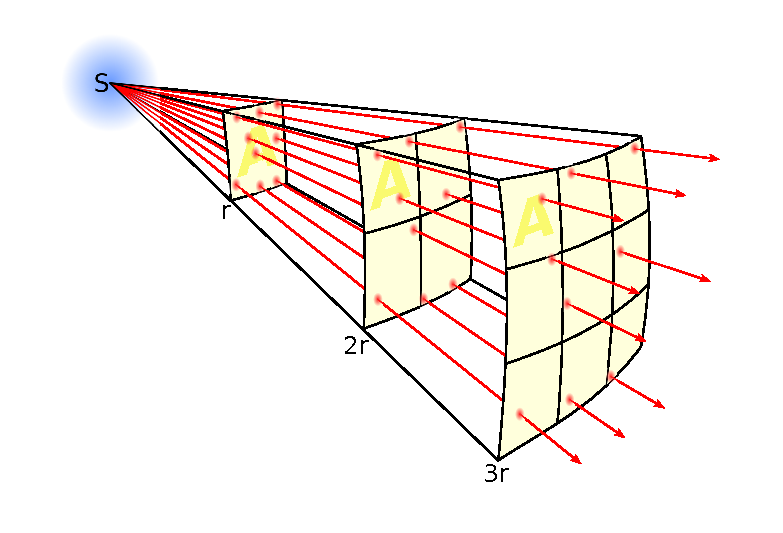
\includegraphics[width=0.5\textwidth]{./fig/photos/Inverse_square_law.eps}
    \caption{An illustration of inverse square law for radiation.\ Source: By Borb, CC BY-SA 3.0, \url{https://commons.wikimedia.org/w/index.php?curid=3816716i}}
      \label{fig:islaw}
  \end{figure}

% %%}

\subsection{Health risk}% %%{
Several health risks are associated with ionizing radiation.
While traversing the human body, ionizing radiation can interact with living tissues causing damage or mutations of individual cells.
In long-term horizon, exposure to ionizing radiation might cause cancer or even genetic disorders.
The severity of health problems depend on exposure time and dose of absorbed radiation.
High doses of ionizing radiation over a short period can cause disease named acute radiation syndrome (radiation sickness).
The disease is manifested by nausea, vomiting, fatigue or even skin burns. 
Depending on the absorbed radioactive dose, it causes several neurological or cardiovascular problems or might lead to death.% %%}






\section{Main types of ionizing radiation}
\subsubsection{Alpha radiation}
Alpha radiation is an emission of positively charged alpha particles consisting of two protons and two neutrons bound together (helium nuclei).
This gives alpha particles a significantly larger mass and higher reactivity compared to other types of ionizing radiation.
On the other hand, they interacts strongly with matter and can't penetrate far.
Alpha particles can travel only few centimeters in air and can be blocked by single sheet of paper or outer layer of human skin.
Because of that, external sources of alpha radiation are generally not considered a significant threat to human health.
The limited range of alpha radiation makes it difficult for sensing from distance.

\subsubsection{Beta radiation}
Beta particles are high-energy, high-speed electrons or positrons.
Due to their smaller size and weaker electrical charge, they are generally more penetrating and less reactive than alpha particles and can reach further in materials.
Several centimeters thick sheet of aluminium or plastic is typically sufficient to block the beta radiation.
In terms of travel through the air, beta particles have range of few meters.
Although the beta radiation is generally less dangerous than gamma, when particles come into contact with human skin, they can penetrate the outer layers and cause skin burns as the particles disrupt cellular processes.

\subsubsection{Gamma radiation}
Gamma rays are often produced alongside alpha or beta particles during radioactive decay. 
Unlike them, gamma radiation of composed of high energy photons. 
They are extremely penetrating and can travel long distances in air as well as get through most of materials or living tissues thanks to their high energy and lack of charge.
Only thick layer of concrete or lead might block this type of ionizing radiation.
These features make the gamma radiation significantly more dangerous than alpha and beta.
The long range of gamma radiation together with negative effects on human health makes it ideal candidate for remote sensing and detection.

  \begin{figure}[!h]
    \centering
      \includegraphics[width=0.6\textwidth]{./fig/photos/pene2.png}
    \caption{Penetrating power of different types of radiation. Source:\url{https://openclipart.org/detail/274074/penetrating-power-of-different-types-of-radiation-alpha-beta-gamma-and-neutrons}}
      %\label{fig:islaw}
  \end{figure}


%On the other hand, ionizing radiation might also have positive impacts on human health.
%It is used in medicine for both diagnostic and therapeutic purposes.

\section{Interaction of $\gamma$ radiation with matter}
Sensing of $\gamma$ radiation is possible through interactions of ionizing photons with imaging devices.
Several interactions might occur when high energetic photon travels through matter, depending on the energy of the incoming photon as well as on the properties of material.
Three main types of interactions are: photoelectric effect, compton scattering and pair production.
The figure \ref{fig:dominant} describes the dominant type of interations depending on the energy of incoming photon and atomic number of the material.

\begin{figure}[!h]
  \centering 

    \includegraphics[width=0.6\textwidth]{./fig/photos/dominant.png}
  \caption{Dominant types of interactions for different energy of photon (x-axis) and atomic number of matrial (y-axis). Source of image: \cite{schwank}}
    \label{fig:dominant}
  
\end{figure}

\subsection{Photoelectric effect and pair production}
In \ac{PE}, also reffered as photoelectric absorbtion, the $\gamma$ photon interacts with orbital electron of absorbing atom.
The photon transfers all its energy to the electron and disappears.
As a consequence, the electron exceeds its binning energy and is emitted from the atom.
The photoelectric absorption is dominant at lower energies of incident photon, however it may occur at any photon energy.
The \ac{PP} occurs only if the $\gamma$ photon has energy exceeding $\approx \SI{1}{\mega\electronvolt}$.
Such very high energetic photon interacts with the nucleolus of the atom.
An electron-positron pair is created as a result of the interaction.

\subsection{Compton scattering}
Third possible interaction (predominant on mid-level energies) is the Compton scattering.
During the Compton scattering, the $\gamma$ photon interacts with an electron loosely bound to the nucleus.
The photon with initial energy $E_{0}$ transfers part of it to the electron.
As a result of the interaction, the lower energetic photon with energy $E_{2}$ is scattered and emitted in direction changed by angle $\beta$. 
The energy difference $E_{1} = E_{0} - E_{2}$ is transferred to a bi-product of the interaction - an electron.
The situation is illustrated in figure \ref{fig:scattering}.

\begin{figure}[!h]
    \centering
    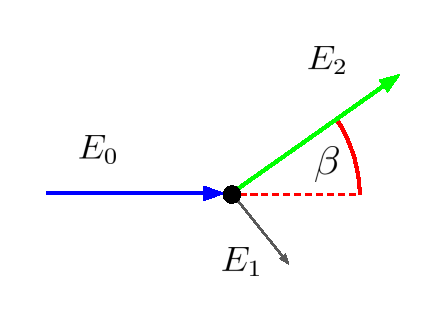
\includegraphics[width=0.3\textwidth]{./fig/photos/compton_simple.eps}
    \caption{An illustration of the Compton scattering. The incident $\gamma$ photon with energy $E_{0}$ (blue) undergoes the Compton scattering. As a result of the interaction, the lower energetic photon (green) with energy $E_{2}$ is emitted under angle $\beta$. Part of the energy ($E_{1}$) is transferred to a bi-product of the interaction- the electron (grey).}
    \label{fig:scattering}
\end{figure}

According to Compton \cite{compton}, the relation of particle energies and scattering angle $\beta$ can be expressed as:

\begin{equation}
E_{2} = \frac{E_{0}}{  1 + (E_{0} / m_{e}c^{2}) (1 - \mathrm{cos} \beta)},
\end{equation}
where $E_{0}$ is the initial energy of the incoming photon, $E_{2}$ is the energy of scattered photon,  $m_{e}$ is the electron rest mass and $c$ is the speed of light in vacuum. 
\mycomment{ %klein nishina % %%{
  The probability that a photon with an energy $E_{0}$ undergoes a Compton scattering through an angle $\beta$ is described by the Klein-Nishina formula
  \begin{equation}
    K(\beta, E_{0}) = \frac{r_{e}^{2}}{2} \left( \frac{E_{2}}{E_{0}}  \right)^{2} \left(  \frac{E_{2}}{E_{0}} + \frac{E_{0}}{E_{2}} - \mathrm{sin}^{2}(\beta)  \right),
    \label{eq:klein_nishina}
  \end{equation}
  where $r_{e}$ is the classical electron radius. 
}% %%}




\section{Measuring radioactivity}
Ionizing radiation is unperceivable by human senses, yet poses a significant health risk for human beings.
Effective monitoring methods are needed to detect and measure a presence of such radiation that is potentially harmful to human beings.
Sensors of ionizing radiation are made of different materials that interact with incoming particles.
Three types of sensors are listed for illustration.
\textbf{Geiger-Müller  counters} are gas-filled tubes, in which the gas is ionized by the passing particles, conducting an electrical charge that can be measured.
\textbf{Scintillation detectors} use a scintillating material that emits light when struck by ionizing radiation.
A photodiode then converts the light to an electrical signal.
Another group of detectors is based on \textbf{semiconductive materials} that are sensitive to ionizing photons. 
The electrons ejected by ionization can be measured and the type and energy of the incoming radiation might be deduced. 

Most of the sensors are simply counting the number of recorded particles and estimates the intensity of particle flux at the given position. 
However, it does not give any information about the direction of incoming particles.
Accurate estimation of distribution of radioactive sources then requires high number of measurements at different positions. 

Following \cite{baca2019timepix}, the direction of incoming particles can be deduced by different detector configurations illustrated in figure \ref{fig:sensor_overview}.
\textbf{Pinhole camera aperture} restricts the field of view by shielding particles from directions other than one narrow passage in the shielding material.
\textbf{Colimators} (frequently used in medical imaging) also restricts the set of possible directions by absorptive material. 
Each part of the detector is responsible for measuring particles coming from certain direction. 
\textbf{Stacked detectors} employ multiple layers, where the particle's direction is computed from interactions at different levels.
Finally, the \textbf{Compton camera} use the Compton scattering for deducing the set of possible directions of the original particle. 




\begin{figure}[!h]
    \centering
    \includegraphics[width=0.5\textwidth]{./fig/photos/detector_overview_baca2019.png}
    \caption{Different ways how to deduce the direction of the incoming particle. Source: \cite{baca2019timepix}}
    \label{fig:sensor_overview}
\end{figure}


\mycomment{
\begin{figure}[!h]% %%{
  \centering
  \subfloat[\centering different ways how to detect the direction of incoming particle. Source: \cite{baca2019timepix}] {
    \includegraphics[width=0.49\textwidth]{./fig/photos/detector_overview_baca2019.png}
    \label{fig:sensor_overview}
  }
  \subfloat[\centering Geometry for two-layer Compton camera. The $\gamma$ particle emitted at position $j$ interacts with the first layer of the sensor (scatterer) at position $X_{1}$. A lower energetic photon is scattered under angle $\beta$ and absorbed by the second layer of the detector (absorber) at position $X_{2}$. The reconstructed Compton cone is parametrized by angle $\beta$, axis vector $a$ and origin of the cone $X_{1}$.] {
      \label{fig:compton_camera_geometry}
  
      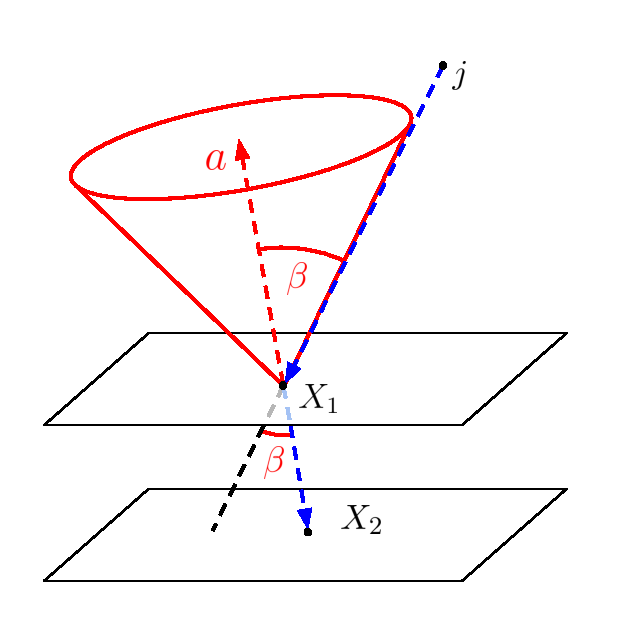
\includegraphics[width=0.49\textwidth]{./fig/photos/compton_camera_modelll.eps}
  }
  \caption{TODO}
  \label{fig:xxx}
\end{figure}% %%}
}


\subsection{Compton Camera}% %%{
The Compton camera is typically composed of two detectors: scatterer and absorber.
The incident photon with energy $E_{0}$ first interacts with the scatterer at position $X_{1}$ in form of Compton scattering.
A bi-product of the interaction (electron with energy $E_{1}$) is immediately captured by the scatterer and its position $X_{1}$ and energy are recorded.
As a result of the interaction, lower energetic photon with energy $E_{2}$ is scattered under (Compton) angle $\beta$.
The scattered photon then interacts in form of \ac{PE} with the absorber.
The absorbed energy $E_{2}$ and the position of the interaction $X_{2}$ are measured and recorded.

The scattering angle $\beta$ can be reconstructed (following \cite{baca2021gamma}) as:
\begin{equation}
  %\beta = \mathrm{arccos} \left (  1-\frac{m_{e}c^{2}E_{2}}{E_{0} (E_{0} - E_{2})} \right )
  \beta = \mathrm{cos}^{-1} 
  \underset{B}{\underbrace{
  \left ( 1+m_{e}c^{2} \left( \frac{1}{E_{1}+E_{0}} - \frac{1}{E_{0}}\right )  \right )
  }},
    \label{eq:compton_beta_formula}
\end{equation}
assuming that $0<B<1$.
Since the Compton scattering is a symmetrical phenomena,  the set of possible directions of incoming particle forms a surface of a cone.
Such conical surface (denoted as Compton cone) is parametrized by the cone axis $a$ (which is a straight line connecting the positions of intersections $X_{1}$ and $X_{2}$), Compton scattering angle $\beta$ and origin of the cone $X_{1}$.
The geometry is illustrated in figure \ref{fig:compton_camera_geometry}.


\begin{figure}[!h]
  \centering
    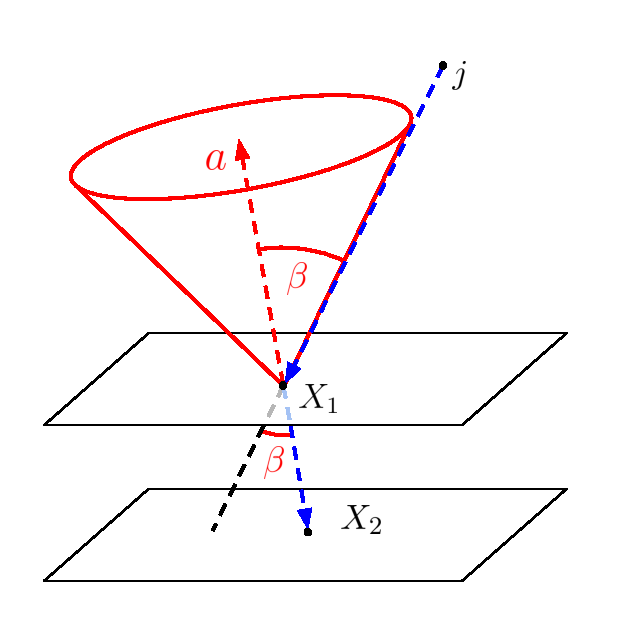
\includegraphics[width=0.4\textwidth]{./fig/photos/compton_camera_modelll.eps}
    \caption{Geometry for two-layer Compton camera. The $\gamma$ particle emitted at position $j$ interacts with the first layer of the sensor (scatterer) at position $X_{1}$. A lower energetic photon is scattered under angle $\beta$ and absorbed by the second layer of the detector (absorber) at position $X_{2}$. The reconstructed Compton cone is parametrized by angle $\beta$, axis vector $a$ and origin of the cone $X_{1}$.}
    \label{fig:compton_camera_geometry}
\end{figure}
% %%}


\section{The MiniPIX TPX3 detector} % %%{
The MiniPIX TPX3 detector\footnote{produced by \textit{Advacam}, https://advacam.com/camera/minipix-tpx3} is a miniature version Timepix3 detector \cite{timepix3}.
It belongs to the class of semiconductor pixel detectors.
The body of the \ac{pix} sensor is made of a compact block of Cadmium telluride (CdTe) semiconductor material with dimensions $14 \times 14 \times 2 \ \si{\milli\meter}$.
Although it has only one detection layer, it can be still used as a Compton camera.

As described in \cite{baca2021gamma} and \cite{baca2019timepix}, the incoming ionizing radiation interacts with the matter of the sensor and separates electrons from the CdTe material.
The newly created electrons are accelerated by a $\SI{450}{\volt}$ electric potential towards one facet of the sensor, where Timepix3 pixel detector is located.
The resolution of pixel detector is $256 \times 256\ \mathrm{px}$, each pixel being $55\ \si{\micro\meter}$ large.
The pixel detector can deduce the energy as well as the type of the absorbed ionizing particle.
Given the measured times of arrival, the coinciding products of Compton scattering might be paired together.
The figure \ref{fig:minipix} depicts the geometry of the \ac{pix} sensor.
The 2D coordinates $\mathbf{\hat{c}}_{x}$,$\mathbf{\hat{c}}_{x}$ (see figure \ref{fig:minipix}) of the interaction are determined by the position of corresponding pixels
The $\mathbf{\hat{c}}_{z}$ coordinate (the depth of interaction in the CdTe block) is unknown.
However, the relative depth position of two coinciding events might be deduced from the times of arrival of the two interactions were captured by the pixel detector.
Because of that, the \ac{pix} detector might be used as a Compton camera.
More technical details related to the sensor operation are provided in \cite{baca2019timepix}.

The \ac{pix} detector has multiple advantages.
It is very compact and lightweight (the size of the whole \ac{pix} sensor is only $80 \times 21 \times 14 \ \si{\milli\meter}$ and it weights $\SI{44}{\gram}$), therefore it can be carried onboard a small \ac{UAV}.
It can report the recorded intersections almost in real time, which allows the to use it for an active strategy, where autonomous \ac{UAV}s react according to the measurements acquired during the flight.

\begin{figure}[!h]
    \centering
  \includegraphics[width=0.5\textwidth]{./fig/photos/minipix.png}
    \caption{An illustration of the detection process inside the MiniPIX TPX3 sensor. Source: \cite{baca2021gamma}}
    \label{fig:minipix}
\end{figure}

\begin{figure}[!h]
    \centering
    \includegraphics[width=0.5\textwidth]{./fig/photos/detector_overview_baca2019.png}
    \caption{different ways how to detect the direction of incoming particle. Source: \cite{baca2019timepix}}
    \label{fig:sensor_overview}
\end{figure}
% %%}



\section{Robot operating system}

\ac{ROS} is a middleware software framework for robotics applications and research.
It follows a distributed architecture with a peer-to-peer communication model.
Individual software modules (called nodes) can exchange data through standardized messages and services.
The communication between \ac{ROS} nodes is maintained by a central authority called \ac{ROS} master.
The \ac{ROS} master provides the registration of the individual \ac{ROS} nodes as well as maintains communication between them.

\subsubsection{ROS messages and topics}
The fundamental \ac{ROS} communication mechanism used for exchanging messages between different \ac{ROS} nodes is called topics.
Topics are based on a publish-subscribe model, where nodes can either publish data to a topic or subscribe to receive data from a topic. 
Each topic has a specific data type associated with it.
Nodes can publish messages of that data type to the topic, and any subscribed nodes will receive those messages.
Topics enable asynchronous communication between different parts of the robotic system, such as data exchange between sensors and onboard computer.

Another important \ac{ROS} communication concept is called service.
\ac{ROS} services allow nodes to make requests and receive responses to them.
Unlike in \ac{ROS} topics, services provides synchronous request-response communication model.
The client node sends its request to a specific service provided by the server node.
The server node processes the request and generates a response message, which is sent back to the sender.
Such communication scheme might be used for example for triggering some action, requesting path from the planning node and generally in any situation where response from the server node is required.

\section{MRS UAV system}
The MRS UAV system \footnote{available at: \url{https://github.com/ctu-mrs/mrs_uav_system}} \cite{mrs_system} is a research-oriented software platform developed at Czech Technical University in Prague.
The consists of the full control pipeline, including state estimation, sensor fusion, trajectory generation, multirobot communication, planning and feedback control.
It enables operations of groups of autonomous \ac{UAV}s in both indoor and outdoor environments.

    
\subsection{Rosbag}
\subsection{architecture}
\subsection{Nodes, Messages and Services}

%%%%%%%%%%%%%%%%%%%%%%%%
%%%%%%%%%%%%%%%%%%%%%%%%%%
%%%%%%%%%%%%%%%%%%%%%%%
%%%%%%%%%%%%%%%%%%%%%%%%%%%%
%%%%%%%%%%%%%%%%%%%%%%%%%%
%%%%%%%%%%%%%%%%%%%%%%%%


\begin{figure}[!h]% %%{
  \centering
  \subfloat[\centering Cross-section for photon interactions in Silicon in the MeV range. The four dominating interaction mechanisms are photo effect, Compton scattering, pair creation and Rayleigh scattering. Source: \cite{zoglauer}] {
    \includegraphics[width=0.2\textwidth]{./fig/photos/cross_stat.png}
    \label{fig:aaaaaa}
  }
  \subfloat[\centering Cross section for compton scattering. Source: \cite{zoglauer}] {

    \includegraphics[width=0.2\textwidth]{./fig/photos/cross_section.png}
    \label{fig:aaaaaa}
  }
  \caption{TODO}
  \label{fig:xxx}
\end{figure}% %%}



\alerterror{Old}% %%{
\mycomment{
  \section{Radioactive decay}
  Radioactive decay is a process where an unstable atomic nucleus transforms into a lower-energy state.
  During this process, it loses energy by radiation.
  There are three main types of such radiation - alpha, beta and gamma.
  Whereas alpha particles can be stopped by a sheet of paper and beta particles by aluminium shielding, gamma particles can be blocked only using a thick block of lead or a massive concrete wall.
  Moreover, highly energetic gamma rays have a negative effect on the human body, causing damage on a cellular level.
  Being exposed to such radiation poses a risk of severe health problems or death.

  \section{Some properties of $\gamma$ radiation}
  \subsection{Inverse square law}
  \subsection{Interaction with matter}

  The quantity of emitted particles ("strength" of the source) is expressed in Becquerels.
  It is a SI unit defined as the number of emitted particles per second.

  \section{Interaction with matter}
  As the gamma particle passes through matter, there are three possible effects that might happen:
  \textbf{the photoelectric effect}, \textbf{Compton scattering} and \textbf{pair production}.

  \textbf{The photoelectric effect} is typical at low energies of gamma rays. A photon undergoes an interaction with an electron that is bound in an atom. The incident photon completely disappears in this interaction. A product of this interaction is a photon.
  \textbf{The Compton effect} is typical for mid-energetic gamma rays. In this process, an incident gamma photon loses energy to an atomic electron. A new lower energetic photon is emitted in a different direction (hence the frequently used term "Compton scattering").
  \textbf{Pair production} is typical for high-energetic gamma rays. It is a process in which a photon of sufficient energy is converted into an electron and a positron.

  The Compton effect (published in 1923 \cite{}) describes the way how a (gamma or X-ray) photon interacts with a static electron. An incident photon with wavelength $\lambda$ losses some energy to the electron. A new lower energetic photon with wavelength $\lambda^{\prime}$ is emitted under angle $\beta$. Thanks to the law of conservation of energy and momentum, Compton derived the following equation
  \begin{equation}
      \lambda^{\prime} = \lambda + \frac{h}{m_{e}c}(1-\mathrm{cos} \beta),
  \end{equation}
  where $\lambda$ is the wavelength of the incident photon, $\lambda^{\prime}$ is the wavelength of the emitted photon, $h$ is the Planck constant, $m_{e}$ is the electron rest mass, $c$ is the speed of light and $\beta$ is the scattering angle.

  \begin{figure}[!h]
      \centering
      \includegraphics[width=0.3\textwidth]{./fig/photos/scattering.png}
      %\label{fig:scattering}
      %\caption{An illustration of Compton scattering. The incident photon interacts with the static electron. As a result, a new lower energetic photon is emitted in a direction changed by $\beta$ as part of its energy is transferred to electron $e^{-}$. Source: \cite{baca2021gamma}}
  \end{figure}


  \subsection{Klein Nishina formula}
  TODO

  \subsection{Compton effect}
  TODO


  \section{Compton camera}
  This effect is the fundamental principle in a sensor called a Compton camera. 
  The sensor is typically composed of two main components: the scatterer and the absorber. 
  The incident photon first interacts with the scatterer, where the lower energetic photon is emitted under angle $\beta$ (thanks to the Compton effect). 
  Since it is more common to measure energies instead of wavelength, we can rewrite the Compton formula as
  \begin{equation}
  E_{\lambda^{\prime}} = \frac{E_{\lambda}}{  1 + (E_{\lambda} / m_{e}c^{2}) (1 - \mathrm{cos} \beta)},
  \end{equation}
  where $E_{\lambda}$ is the energy of the incoming photon from the source, $E_{\lambda^{\prime}}$ is the energy of the scattered photon.  
  The bi-product of the interaction (electron $e_{e^{-}}$) is immediately measured in the scatterer, and its position is recorded.
  Then, the scattered lower energetic photon interacts with the second layer of the sensor - the absorber. 
  The photoelectric effect is witnessed while measuring the product of it - the energy of the electron $e_{\lambda^{prime}}$ and its position on the absorber.

  Now we can express the scattering angle $\beta$ as
  \begin{equation}
      \beta = \mathrm{arccos} \left (  1-\frac{m_{e}c^{2}E_{\lambda^{\prime}}}{E_{\lambda} (E_{\lambda} - E_{\lambda^{\prime}})} \right )
      %\label{eq:compton_beta_formula}
  \end{equation}

  Given the measurements on the scatterer and absorber and computed scattering angle $\beta$ using the equation \ref{eq:theta} (using known energy of the incoming photon $E_{\lambda}$), we can reconstruct a set of possible directions from where the original photon arrived. Since the Compton effect is symmetrical, the set of possible directions towards the source of ionizing radiation forms a surface of a cone.



  \subsection{MiniPIX TPX3 sensor}
  The sensor used in this work is a small CdTe event-based camera that is capable of witnessing the interactions between gamma photons and the matter of the sensor and reporting them in real time.
  Unlike the traditional model of the Compton camera mentioned before, this is a single-stack detector.
  In other words, there is no distinction between the scatterer and the absorber and all the measurable interactions are happening in one 14x14x2 mm block of CdTe semiconductor material.
  The sensor is capable of measuring a 3D position of the interactions (and distinguishing its type) inside the detector with nanosecond resolution. 
  All these features open the possibility of using it in Compton camera mode.
  Technical details of the sensor are described in \cite{baca2021gamma} and \cite{baca2019timepix}.
  The biggest advantage of this sensor is its small size, low weight and low power consumption.
  Thanks to that, we can use this sensor on board a small UAV. 


  \section{Cs137}

  \section{ROS}

  \section{MRS UAV system}
}
% %%}

%!TEX root = ../main.tex
\chapter{Methods for compton camera image reconstruction}
The 3D reconstruction of sources of ionizing radiation poses a challenging problem.
The difficulty of this task lies in the fact that the detected $\gamma$ particle could originated anywhere on the surface of the reconstructed compton cone.
Several methods for compton imagining have been investigated in the past.
This chapter provides a brief overview of such methods.

\section{Compton imagining in nuclear medicine}
The problem of reconstructing 3D positions of sources of ionizing radiation has been studied in depth in the field of medical imagining.
It is used as a non-invasive method for diagnostics.
To give an example:
In cancer diagnostics, small amount of radioactive substance (called tracer) is injected into the patient's vein.
The tracer is absorbed by different parts of the body in varying amounts, which can show areas with abnormal metabolic activity, which is usually the case for cancer cells.
The detection of emitted particles and 3D reconstruction of their sources allow doctors to find the location of the tumor in the patient's body.

\section{Differences}
Such medical application typically requires high resolution of the reconstructed image.
The distances between the source and detector are small (tens of centimeters), number of measured events is high (tens of thousands and more).
The reconstruction process is typically performed offline (all measurements are collected first and then the algorithms process the data), since there is no need for online estimation and the processing of measured data might take non-negligible time.
The domain of multirobotic radiation mapping has multiple differences compared to the medical field.
The distance between source and detector is much higher (from meters to tens of meters).
The \ac{UAV}s have limited payload (hence the detector carried on board must be light and compact).
It results in the fact that the number of measurements is much lower (hundreds-thousands detected compton events).
Moreover, we would like to reconstruct the sources of ionizing radiation in real time.
Despite all of these differences, the aim of this work is to get inspiration in the medical field and apply these algorithms to the given problem.

\section{Analytical and iterative methods}
Literature describes two main categories of reconstruction methods: analytical and iterative algorithms \cite{lojacono2}.
In analytical methods, the aim is to find solution directly from the conical projections of reconstructed Compton events.
Such solution might be exact in the continuous model, yet impractical in real world applications, where the measurements might be noisy (thus conical surface projections might not intersect the real position of the source) or where the computational power is limited.

To illustrate difficulties of direct reconstruction methods, algorithm proposed in \cite{baca2021mrs} estimates the initial hypothesis of the source position as a point that is closest to all measured cone surfaces (which might be considered as analytical method).
Finding solution of such non-linear least squares problem is computationally demanding and tractable only for small number of cones.
Another example of simple analytical method is called backprojection.
It can be used as follows:
the detection space is divided into discrete bins.
For each Compton measurement, the cone surface is backprojected to the discrete bins.
The intersection of the cone with the bins is recorded.
The bins with higher number of intersections presents possible locations of $\gamma$ particles sources.

The iterative algorithms work with discretized space.
These methods  approximate the positions of sources by iteratively adapting the reconstruction to the measured projections.
This approach do not provide exact and unique solution, on the other hand it is more flexible, can handle noise in the measurements (if it is properly modelled) and is widely used in practise \cite{lojacono2}.

Literature describes there main methods: \ac{MLEM}, \ac{MAP} and \ac{SOE}.
\ac{MLEM} (\cite{MLEM_Shepp_1982}, \cite{MLEM_Lange_Carlson_1984}, \cite{MLEM_Wilderman_2000}) is an iterative algorithm that is based on the maximum likelihood approach.
This classical method is widely used for image reconstruction from \ac{CC} data \cite{maxim2016}.
Another approach called \ac{MAP} \cite{MLEM_Lange_Carlson_1984} is based on bayesian approach.
It is an extension of \ac{MLEM} that allows to incorporate some prior knowledge about the source distribution or features of the data.
\ac{SOE} is a stochastic algorithm that randomly assigns origins of the measured events to the conical surfaces.
During the course of reconstruction, the origins of events are stochastically moved and the acceptance of the new event origin is determined by the change in event density.
After several iterations, the reconstructed distribution of origins converges to a quasistationary state \cite{SOE_Andreyev_2009}.

The iterative methods were originally developed for \ac{PET} and \ac{SPECT} imagining.
The \ac{PET}  method is based on positron emission. 
The emitted positron interacts with electron in the patients body and both particles vanish in a burst of energy. 
This energy comes in a form of two gamma rays, that goes into a opposite directions.
Detection of these two gamma rays (measured by the camera at the same time) allows us to reconstruct 3D image of the patient's body.
In \ac{SPECT}, only a single gamma ray is produced. 
Medical \ac{SPECT} imagining devices typically acquire measurements from different positions and use collimators to restrict the set of possible directions of incoming gamma ray.
Measured events in \ac{PET} and \ac{SPECT} are stored in memory in discrete bins (each bin represents count of reconstructed particles in defined time interval or subset of the image space).
On the other hand, the \ac{CC} events are represented in memory using List-mode approach.
It is a list data structure, where each record contains information about the exact arrival time, position and energy of measured interactions useful for Compton cone reconstruction.
Despite all these differences in the nature of the measurements, the methods were adapted for Compton imagining as well.

%Collimators restricts the set of possible directions from which the gamma ray may enter the detector (and be detected), therefore they can improve accuracy of the detection.
%Since only one gamma-ray is emmited (unlike in \ac{PET}), high number of measurements is needed for accute reconstruction.
%Medical \ac{SPECT} imagining cameras typically use collimators to get some information about direction of incoming gamma ray.
%Collimators restricts the set of possible directions from which the gamma ray may enter the detector (and be detected), therefore they can improve accuracy of the detection.

\section{Maximum likelihood expectation maximization}
The description of the \ac{LM-MLEM} algorithm is given in this section.
It was originally proposed by \cite{1982_shepp_vardi_MLEM} and later adapted to \ac{CC} data and list-mode form by \cite{wilderman}.

\subsection{Maximum likelihood estimation}
\ac{MLE} is a classical approach in machine learning.
It is used to estimate the parameters of a probability distribution based on observed data. 
The goal of \ac{MLE} is to find the parameter values that make the observed data most probable under the assumed probability distribution.
This is done by calculating the likelihood function, which is the probability of the observed data given a set of parameter values.
Likelihood can be defined as 
\begin{equation}
  \mathcal{L}(\boldsymbol{O}| \Phi) = p(\ \mathrm{observing\ measurements} \  \boldsymbol{O} \ \mathrm{given\ parameters\ } \Phi ).
  \label{eq:likelihood}
\end{equation}
We want to maximize this expression with respect to the hidden parameters.
In other words, we want to find such parameters so that they fit our observations in the best possible way.

\subsection{Original MLEM formulation}
Let's divide the area of possible sources of radiation into $J$ discrete bins (indexed with $j$, where $j = 1 \dotsc J$).
Each discrete bin is represented by its center position.
Suppose the binned data space of all measured events is $\mathbf{I}$, divided in $I$ discrete bins indexed with $i$, $i = 1 \dotsc I$.
The unobservable data space of all not measured events is denoted $\mathbf{\hat{I}}$.
The vector $\mathbf{Y}$ with elements $y_{i}, i \in (1, \dots I)$ denotes the number of particles detected in the corresponding bin $i$.
%(the algorithm was originally developed for \ac{PET} imaging, where $y_{i}$ can be arbitrary number, $y_{i} = 1$ in list-mode representation).
Let's define matrix $\mathbf{T}$ ($\mathbf{T} \in \mathbb{R}^{I \times J}$), where each position in the matrix is defined as

\begin{equation}
  t_{ij} =  P(\textrm{detected in } i | \textrm{emitted from } j).
\end{equation}

In other words, $t_{ij}$ represents a probability that we observe observation $i$ given the fact that a radioactive particle was emitted from position $j$.
Lets assume that we know the matrix $\mathbf{T}$.

Let's assume that the number of photons emitted from one position $j$ is a discrete random variable that follows a Poisson distribution with expected value $\lambda_{j}$.
Our goal is to estimate $\mathbf{\lambda}$, which has elements $\lambda_{j}$, each corresponding to the expected intensity of emission from the position $j$.
Then a vector $\mathbf{M}$ can be defined, where each element of $\mathbf{M}$ 
\begin{equation}
  \mu_{i} = \sum_{j} t_{ij}\lambda_{j}
  \label{eq:mu}
\end{equation}
denotes the average number of events measured in bin $i$.

The probability of measuring $y_{i}$ particles in the measurement bin $i$ w.r.t. to some given $\mathbf{\lambda}$ can be expressed as (Poisson distribution):
\begin{equation}
  p(y_{i} |\mu_{i} ) = e^{-\mu_{i}} \frac{\mu_{i}^{y_i}}{y_{i}!},
\end{equation}

The likelihood of all the measurements (assuming the events to be independent) is
\begin{equation}  
  \mathcal{L}(\mathbf{Y} | \mathbf{\lambda}) = \prod_{i}p(y_{i} |\mu_{i} ) = \prod_{i} e^{-\mu_{i}} \frac{\mu_{i}^{y_i}}{y_{i}!}.
\end{equation}

Instead of maximizing the product, it is natural to maximize its logarithm, since the logarithm is monotonically increasing function.
After taking its logarithm and substituting \ref{eq:mu}, we have the following:
\begin{equation}  
  \mathrm{log}\ \mathcal{L}(\mathbf{Y} | \mathbf{\lambda}) = \sum_{i}\left ( -\sum_{j} t_{ij}\lambda_{j} + y_{i} \mathrm{log}(\sum_{j} t_{ij}\lambda_{j})  - \mathrm{log}(y_{i}!) \right ).
  \label{eq:likelihood1}
\end{equation}
Then the maximum likelihood solution of the given problem is
\begin{equation}
  \mathbf{\lambda}_{best} = \underset{\mathbf{\lambda}}{\mathrm{argmax}}( \mathrm{log}\ \mathcal{L}(\mathbf{Y} | \mathbf{\lambda}))
\end{equation}
However, the nonlinear equation \ref{eq:likelihood1} can not be maximized directly.
The solution is to use an iterative \ac{EM} algorithm, as proposed in \cite{MLEM_Lange_Carlson_1984}.
\subsection{Expectation maximization algorithm}
The \ac{EM} algorithm was originally developed by \cite{EM}. 
It is an iterative algorithm consisting of two steps performed in each iteration - E-step and M-step.
Lets denote $l$ the number of iteration of the algorithm.
The vector of hidden parameters $\mathbf{\hat{\lambda}}^{[l = 0]}$ is initialized to some starting value using back-projection of the compton cones.

The purpose of the E-step is to determine the expectation of the likelihood function given the measurements $\mathbf{Y}$ and the estimation of hidden parameters $\mathbf{\hat{\lambda}}^{[l-1]}$ obtained from the previous iteration. 
Then in the M-step, this expectation is maximized by setting its derivatives w.r.t. $\mathbf{\hat{\lambda}}^{[l-1]}=0$.
According to \cite{MLEM_Lange_Carlson_1984}, the final formula for iterative \ac{MLEM} algorithm with binned data is 
\begin{equation}
  \hat{\lambda}_{j}^{[l]} = \frac{\hat{\lambda}_{j}^{[l-1]}}{\sum_{i}t_{ij}} \sum_{i \in I} \frac{t_{ij} y_{i}}{\sum_{k} t_{ik} \hat{\lambda}_{k}^{[l-1]}}.
  \label{eq:mlem_class}
\end{equation}
The term $\sum_{i}t_{ij}$ is called sensitivity of detection $s_{j}$ and presents a probability that particle emitted at position $j$ is detected by the sensor:
\begin{equation}
  s_{j} = P(\textrm{detected by the sensor}\ | \textrm{emitted from } j) =  \sum_{i}t_{ij}
\end{equation}

\subsection{List-mode Maximum Likelihood Expectation Maximization}
The List-mode extension of \ac{MLEM} for \ac{CC} imaging was proposed in \cite{wilderman}.
Each measurement bin in \ac{LM-MLEM} is consisting of only one detected Compton event.
Therefore the number of detected events $y_{i}$ in data bin $i$ is either $y_{i} = 1$ for detected event or $y_{1} = 0$ when no event was recorded.
This simplifies the formula \ref{eq:mlem_class} to

\begin{equation}
  \hat{\lambda}_{j}^{[l]} = \frac{\hat{\lambda}_{j}^{[l-1]}}{s_{j}} \sum_{i \in \mathbf{I}}\frac{t_{ij} }{\sum_{k} t_{ik} \hat{\lambda}_{k}^{[l-1]}}.
  \label{eq:lmmlem}
\end{equation}

Since only recorded measurements are considered in the list-mode approach, it no longer holds that sensitivity of measurements can be expressed as $s_{j} = \sum_{i}t_{ij}$ (summation over all measurement bins $i$).
The sensitivity of detection is a sum over all events, not only those that were measured, therefore 

\begin{equation}
s_{j} = \sum_{\mathbf{I} \cup \mathbf{\hat{I}}} t_{ij} 
\end{equation}
for \ac{LM-MLEM}.

\subsection{LM-MLEM in practical application}
The equation \ref{eq:lmmlem} presents the formulation of iterative algorithm maximalizing the likelihood of measured data.
The system matrix $\mathbf{T}$ and vector of sensitivity values $\mathbf{S} \in \mathbb{R}^{J}$ with elements $s_{j}$ depend on the particular geometry of the used sensor and need to be derived individually in each application.
%Another design-choice is the initialization of the vector $\mathbf{\hat{\lambda}}^[l = 0]$.



%Since the data for \ac{CC} are stored using list-mode approach, the $y_{i}$ (number of detected events in data bin $i$) in equation \ref{eq:mlem_class} is either $0$ or $1$.


\section{The algorithm of choice}
The choice of reconstruction method for the given task (estimation of sources locations from \ac{CC} measurements acquired by a group of \ac{UAV} equipped with \ac{pix} detector) was made under following assumptions.
The iterative methods are more flexible and can handle noise in the measurements.
The distance between the source and \ac{CC} onboard the \ac{UAV}s is high and the number of measured events (represented using list-mode approach) is relatively low.
There is no prior knowledge about the distribution of radioactive sources.
The \ac{CC} data are represented using list-mode approach.

%\section{Imagining in nuclear medicine}
%The problem of reconstructing 3D positions of sources of ionizing radiation has been studied in depth in the field of medical imagining.
%To give an example: one possible application of such methods is a cancer diagnostics.

%There are numerous methods used in medical imagining. 
%Two main approaches are following: \ac{PET} and \ac{SPECT}.
%\ac{PET} imagining typically use a gamma emitting radioisotope as a tracer.  
%The method is based on positron emission. 
%The emitted positron interacts with electron in the patients body and both particles vanish in a burst of energy. 
%This energy comes in a form of two gamma rays, that goes into a opposite directions.
%Detection of these two gamma rays (measured by the camera at the same time) allows us to reconstruct 3D image of the patient's body.
%In \ac{SPECT}, single gamma ray is produced. 
%The reconstructed image is computed from gamma rays detected by the camera.
%Since only one gamma-ray is emmited (unlike in \ac{PET}), high number of measurements is needed for accute reconstruction.
%Medical \ac{SPECT} imagining cameras typically use collimators to get some information about direction of incoming gamma ray.
%Collimators restricts the set of possible directions from which the gamma ray may enter the detector (and be detected), therefore they can improve accuracy of the detection.

%Another type of sensor (that can be used in \ac{SPECT} imagining) is a Compton camera.
%The biggest benefit of compton camera is that it provides information about the direction of detected incoming gamma ray without the use of collimator.
%The nuclear medicine reconstruction method for compton camera measurements that served as inspiration for for this thesis is called \ac{LM-MLEM}.

%!TEX root = ../main.tex
\chapter{Compton imaging for a group of UAVs\label{chap:methods_estimation}}
The \ac{MLEM} algorithm for Compton imaging described in the previous chapter has been chosen as a suitable method for data fusion of Compton measurements acquired by a group of \ac{UAV}s.
The motivation for the use of \ac{MLEM} method is described in section \ref{sec:prelim}.
Section \ref{sec:setup} presents the adaptation of \ac{MLEM} to the task of online estimation performed by a group of \ac{UAV}s.
The definition of sensitivity and system matrix is described in sections \ref{sec: sensitivity} and \ref{sec:system}.

\section{The algorithm of choice}
\label{sec:prelim}
The algorithms for Compton imaging in nuclear medicine (described in the previous chapter) served as inspiration for the imaging method proposed in this thesis.
The algorithm of choice is \acf{MLEM} (more precisely, its list-mode variant for Compton imaging) for the following reasons.

Firstly, the maximum likelihood approach allows us to model factors influencing the measurements (such as air attenuation, the distance between the source and the sensor of ionizing radiation,  properties of the sensor and random processes leading to the detection)
as well as cope with the stochastic nature of radioactive emission and model both in a probabilistic way.
It is also a relatively easy-to-apply and time-proven method in the field of nuclear medicine, which has been applied in the robotic sensing of ionizing radiation.

Secondly, the \ac{MLEM} can take into account not only ``positive'' measurements (the Compton events recorded by the sensor) but also ``negative'' measurements (meaning what was NOT measured by the sensor at the given position in space).
Although the radioactive emission, as well as Compton event detection, are stochastic processes, the fact that an \ac{UAV} flew over some position multiple times and did not measure any Compton event is valuable information that might help improve the estimate.
The sensitivity of detection (that is computed during the steps of \ac{MLEM} algorithm) might serve as a map of coverage of the monitored area.
In other words, the sensitivity of detection provides information about how well was which part of the area explored by the drones equipped with the Compton cameras.

Lastly, the algorithm can be easily applied in a scenario with multiple \ac{UAV}s equipped with Compton cameras.
The \ac{MLEM} method is also computationally tractable under some assumptions 
(such as a relatively low number of detected events (which holds for the given scenario and type of sensor) or restriction on the set of possible sources locations)
and can be evaluated online.
The almost real-time estimation is important for active search strategy, where the \ac{UAV}s may adapt to the current situation and optimize the search strategy.

\section{Online MLEM Compton imaging for group of \ac{UAV}s}
\label{sec:setup}
\subsection{Discretization and hidden parameters}
As described in the chapter \ref{chap:mlem_theory}, the \ac{MLEM} algorithm belongs to the class of iterative algorithms that work with discretized space of possible source locations.
We assume that the source of ionizing radiation is static and located somewhere on the ground.
We further assume that the \ac{UAV}s are exploring a flat outdoor area without obstacles. Therefore all the potential sources of ionizing radiation are located somewhere on the flat 2D ground plane.

The area of interest (where possible sources of ionizing radiation might be located) is divided into $J$ discrete bins with resolution $r$, each of them is approximated by its centre position and indexed with $j$, $j \in \{1, \dots , J\}$.
The set of all collected measurements (the Compton cones) is denoted $\mathbf{I}$.
The Compton cones are indexed with $i$, $i \in \{1, \dots, I\}$, where $I$ is the total number of cones recorded.
The vector of hidden parameters $\bm{\lambda}\in \mathbb{R}^{J}$ is defined analogously as in the previous chapter, where each element $\lambda_{j}$ represents the expected value of the Poisson distribution, specifying the expected emission rate at position $j$.
The discretization process is illustrated in figure \ref{fig:discretization}.

%multifigure discretization%%{
\begin{figure}[!h]
  \centering

  \subfloat[area of interest] {
    \includegraphics[width=0.32\textwidth]{./fig/photos/dis1.eps}
    \label{fig:dis1}
  }
  \subfloat[area discretized with resolution $r$] {
    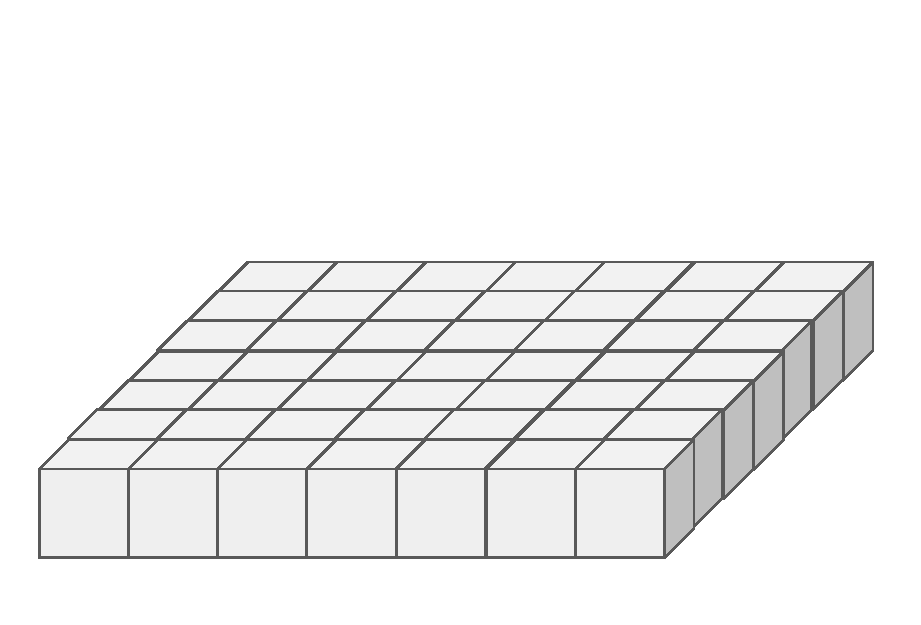
\includegraphics[width=0.32\textwidth]{./fig/photos/dis2.eps}
    \label{fig:dis2}
  }
  \subfloat[hidden parameters $\bm{\lambda}$] {
    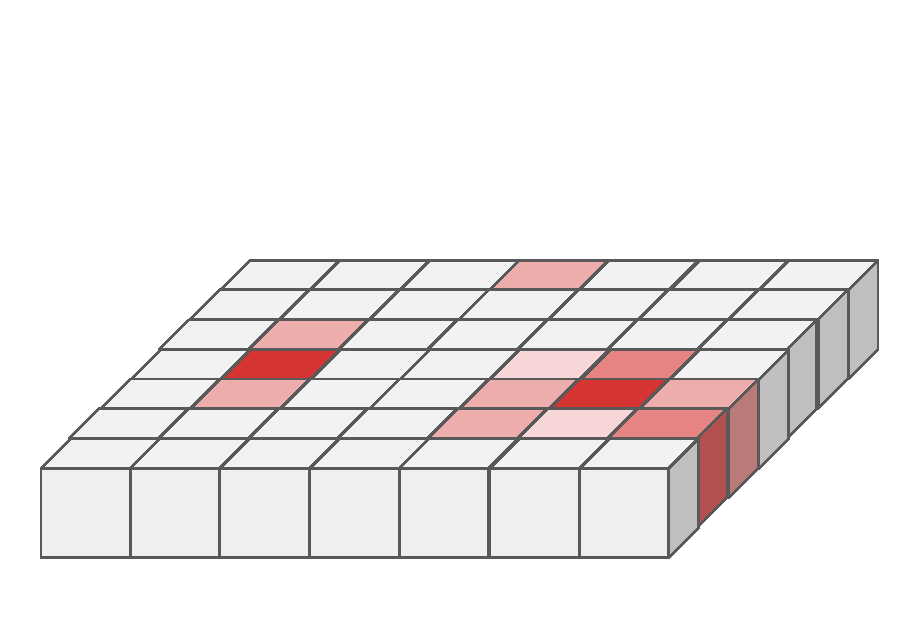
\includegraphics[width=0.32\textwidth]{./fig/photos/dis3.eps}
    \label{fig:dis3}
  }
  \caption{Illustration of the discretization of the space of possible source positions. The open area without obstacles (\ref{fig:dis1}) is discretized into $J$ discrete bins (\ref{fig:dis2}), each represented by its centre position and associated with hidden parameter $\lambda_{j}$ (\ref{fig:dis3}).}
  \label{fig:discretization}
\end{figure}% %%}

\subsection{Online maximum likelihood estimation}% %%{
The estimation process proceeds iteratively using the list-mode \ac{MLEM} algorithm:
\begin{equation}
  \lambda_{j}^{[l]} = \frac{\lambda_{j}^{[l-1]}}{s_{j}} \sum_{i \in I} \frac{t_{ij}}{\sum_{k} t_{ik} \lambda_{k}^{[l-1]}},
  \label{eq:MLEM}
\end{equation}
where $l$ is the current iteration of the algorithm, $\lambda_{j}$ is the hidden parameter for each position $j$ we would like to estimate, $t_{ij}$ is the element of system matrix $\mathbf{T}\in \mathbb{R}^{I \times J}$ and $s_{j}$ is the sensitivity of detection for the map position $j$.

As stated before, the \ac{MLEM} algorithm is typically used as an offline method that proceeds all the measurements at once after the end of the experiment.
Medical applications with highly sensitive detectors, together with the short distance between the source and the detector, produce a large number of measurements (tens of thousands and more), and the algorithm typically reconstructs the 3D space with high resolution.
The high number of Compton events results in the fact that the $\mathbf{T}\in \mathbb{R}^{I \times J}$ cannot be stored in the memory during the run of the algorithm and its individual elements $t_{ij}$ are recomputed in every step of the algorithm, which significantly prolongs the computing time.
If the instance of the problem (size of the sampled space $J$ and the number of measurements $I$) is reasonably small, the system matrix $\mathbf{T}$ can be computed only once for each measurement and stored in the memory for future computations, which speeds up the future runs of the \ac{MLEM} algorithm.
Furthermore, the iterations of the \ac{MLEM} algorithm reformulated as matrix multiplication are parallelized using \ac{GPU}.

Figure \ref{fig:online_mlem} depicts the workflow of \ac{MLEM} estimation during the experiment.
As the drones fly through the environment, each of them samples its current position at $\SI{5}{\hertz}$.
The sensitivity of detection vector $\mathbf{s}\in \mathbb{R}^{J}$ is updated online based on the newly sampled positions.
Once the new measurement (Compton cone) $i$ is detected, the vector $\mathbf{t}_{i} = [t_{i0}, \dots,t_{ij}, \dots, t_{iJ}]$ is appended to the system matrix.
The iterative \ac{MLEM} algorithm (\ref{eq:MLEM}) is then repeatedly computed (at $\SI{0.5}{\hertz}$) using currently available sensitivity vector $\mathbf{s}$,  system matrix $\mathbf{T}$ and initialized vector of hidden parameters $\bm{\lambda}$.
The estimate of the distribution of radioactive sources $\bm{\lambda}$ is therefore updated every $2$ seconds, which is technically speaking not in real-time, but the update frequency is sufficient for planning the next actions of the \ac{UAV}s based on the measured data.
%The vector $\bm{\lambda}^{[l=0]}$ is initialized with uniform distribution
%Experiments showed that the proposed approach is computationally tractable for scenarios with an area of size $300 \times 300\ \si{\meter}$ and number 
\mycomment{% %%{
Experiments in simulation and also in real-world showed that the assumption of reasonably small instances holds in practice for the proposed application.
The proposed method is 


The sensitivity vector $\mathbf{s}$ can be iteratively updated during the experiment and with constant memory requirements since the individual elements $s_{j}$ can be updated in place.

The sensitivity vector $S$ is iteratively updated using recorded drone positions that are sampled from drone trajectories (with frequency $\SI{5}\hertz$).
The details of sensitivity computation is provided in section \ref{sec: sensitivity}.
The system matrix $\mathbf{T}$ is updated (a new row is added) every time a new Compton cone is detected.
The estimation of system matrix $\mathbf{T}$ is described in section \ref{sec:system}.

The iterative \ac{LM-MLEM} algorithm described in equation \ref{eq:MLEM} is processed regularly.
The vector of hidden parameters $\mathbf{\Lambda}$ is initialized with cones back-projection.
The \ac{LM-MLEM} estimate is recomputed every $2$ seconds.
}% %%}
% %%}
%figure melm online%%{
\begin{figure}[htb]
  \centering
    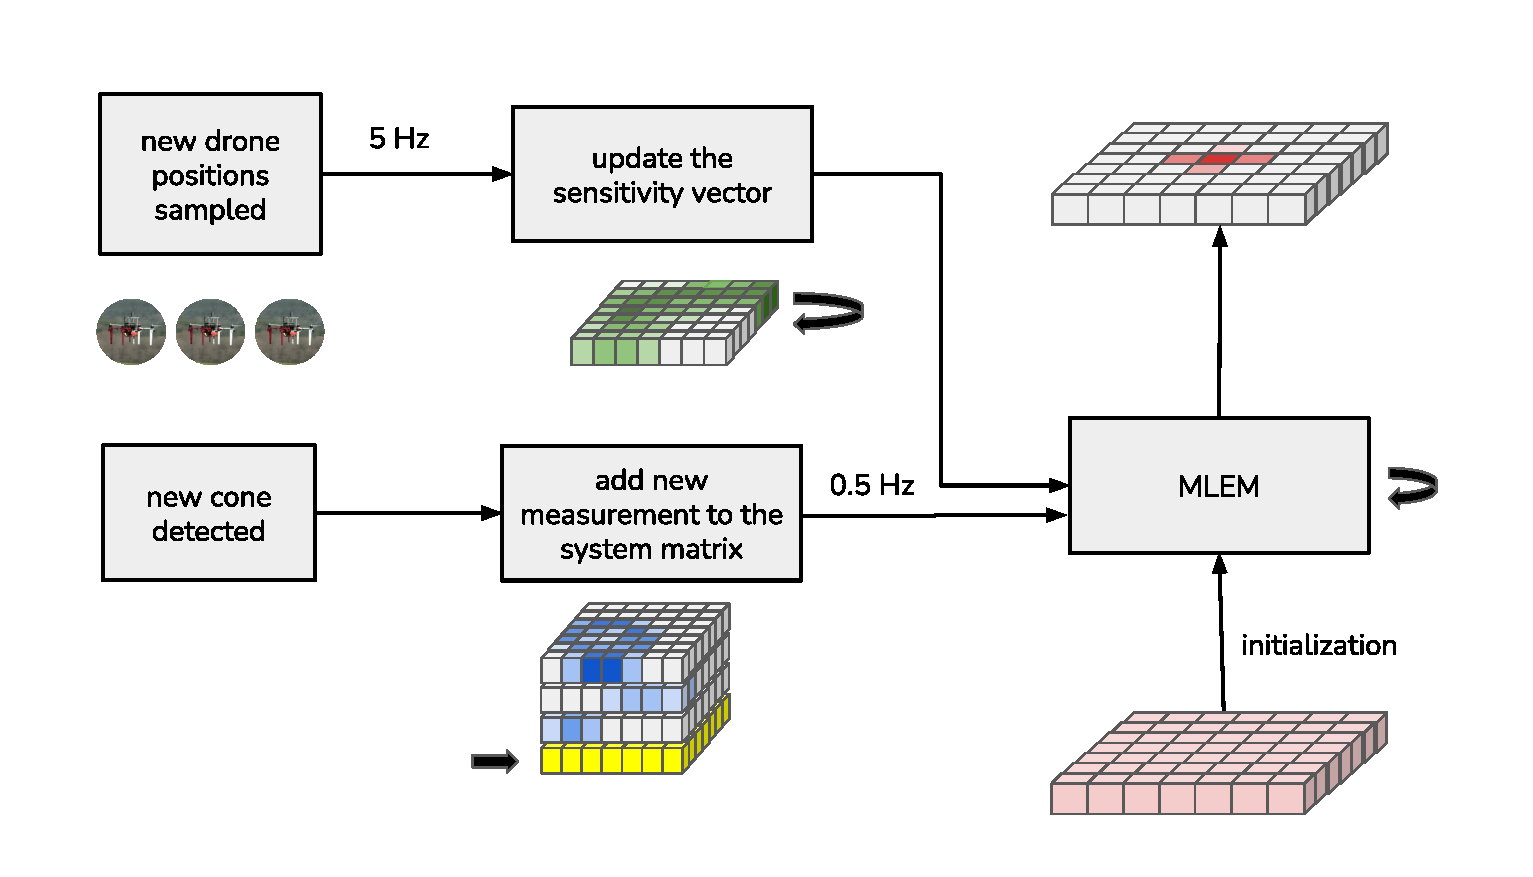
\includegraphics[width=0.99\textwidth]{./fig/photos/workflow.eps}
  \caption{Workflow of the (almost) real-time \ac{MLEM} estimation. The positions of \ac{UAV}s are sampled at $\SI{5}{\hertz}$ and the sensitivity vector $s$ (green) is updated online based on newly sampled positions.
  Once the new Compton cone $i$ is detected by the \ac{pix} Compton camera, 
  the matrix $\mathbf{T}$ (blue) is extended by the new vector $\mathbf{t}_{i} = [t_{i0}, \dots,t_{ij}, \dots, t_{iJ}]$ (yellow).
  The iterative \ac{MLEM} algorithm then computes the current estimate of emission intensity $\bm{\lambda}$ (red) every $2$ seconds.
  }
    \label{fig:online_mlem}
\end{figure}% %%}

%Experiments showed that the proposed approach is computationally tractable for real-world scenarios 
%(e.g. autonomous search for multiple compact sources of ionizing radiation of activity $\approx \SI{10}{\giga\becquerel}$ located somewhere in area of size $300 \times 300 \si{\meter}$ discretized with resolution $r = \SI{1}{\meter}$).
%However, there might be scenarios 
%The computational complexity of the \ac{MLEM} algorithm is $\mathcal{O}(I \ J)$, where $I$ is the number of measurements and $J$ is the number of map positions.
%The memory requirements are $\mathcal{O}(I \times J)$
%The scalability of the proposed solution depends on the number of measured Compton cones ($I$) and the size of the area of interest ($J$).
%The number of 
%Experiments showed that the proposed approach is computationally tractable for real-world scenarios 
%(e.g. autonomous search for multiple compact sources of ionizing radiation of activity $\approx \SI{10}{\giga\becquerel}$ located somewhere in area of size $300 \times 300 \si{\meter}$ with sampled with resolution $r = \SI{1}{\meter}$  
%
%The computational feasibility has been tested in simulations and in real-world experiments.

%The sensitivity of detection as well as the system matrix is defined in the following sections.
%The assumption of a reasonably small scenario holds for the proposed application, 
%where the number of recorded Compton cones $I$ is of the order of $10^{3}$ 
%(given low sensitivity and small size of the \ac{pix} sensor) 
%and size of the discretized mapped area $J$ of the order of $10^{5}$  (e.g. area of $300 \times 300 \si{\meter}$ with resolution $r = \SI{1}{\meter}$).

\section{Sensitivity of detection}% %%{
\label{sec:sensitivity}
The probability of a photon emitted from a given position $j$ to be detected by the Compton camera is called the sensitivity of detection.
It can be expressed using conditional probability as 
\begin{equation}
  s_{j} =  P(\textrm{detected by the sensor}\ | \textrm{emitted from } j).
\end{equation}
A series of random occurrences should happen for a photon to be detected by the Compton camera.
First of all, the photon must be emitted from position $j$ towards the sensor surface (emitted under the solid angle subtended by the visible camera surface at the position of the source), not being absorbed by the air along the way.
Then the photon should interact with the matter of the sensor in form of Compton scattering.
%The angle under which it scatters can be described by the Klein-Nishina \cite{Klein-Nishina cross-section.
The scattered photon then must be absorbed by the camera in the form of a photoelectric effect.
This model is simplified because other random occurrences might happen --- for example, the photon might undergo Compton scattering twice in a row, the incident photon might be immediately absorbed, etc.
However, we will stick to the proposed simplified model with particles undergoing Compton scattering and then photoelectric absorption consecutively.

The position of the Compton camera sensor is not static in this case. 
The \ac{UAV}s carrying the Compton camera are dynamically moving through the environment, with varying speed, position and orientation.
Therefore, the positions of the \ac{UAV}s are sampled in time from \ac{UAV}s trajectories and denoted as $v$, where $v \in \{0, \dots , V\}$ and $V$ is the total number of viewpoints generated by all \ac{UAV}s during the experiment.
The sensitivity of detection is evaluated for each $(j,v)$ pair. % %%}

\begin{figure}[!h]
  \centering
    \includegraphics[width=0.65\textwidth]{./fig/photos/sen.eps}
    \label{fig:sen_illustration}
  \caption{An illustration of sensitivity computation. The sensitivity describes the probability that a particle emitted at a given position is measured by the Compton cameras onboard the \ac{UAV}s. In other words, the sensitivity $s_{j}$ describes how well explored has been the map position $j$ during the experiment. The trajectory of the \ac{UAV} is sampled into viewpoints denoted as $v$.}
\end{figure}% %%}

\subsection{Probabilistic description}% %%{
The series of random occurrences for a photon emitted at position $j$ leading to the detection by the Compton camera at camera position $v$ can be described as follows:
\begin{equation}
  s_{jv} =  (p_{solid\ angle})(1-p_{air})(p_{compton})(p_{absorption}),
  \label{eq:sen_prob}
\end{equation}
where $p_{solid\ angle}$ is the probability that the photon is emitted under the solid angle subtended by the visible camera surface (at position $j$), 
$p_{air}$ is the probability that a photon is absorbed by the air along the way from emission towards the sensor, 
$p_{compton}$ is the probability that Compton scattering occurs, and $p_{absorption}$ denotes that scattered photon is absorbed by the detector and measured.

The literature describes several analytical models for computing the sensitivity of the detection. 
For example, \cite{wilderman2001} proposed a sensitivity model for multi-layer Compton cameras close to the source.
Authors of \cite{maxim2016} proposed a simplified model for Compton cameras with negligible size compared to the distance from the source.
However, these models are not suitable for the problem tackled in this thesis since the multi-layer Compton camera has different properties than the single-layer Compton camera \ac{pix}.
Multi-layer Compton cameras are typically measuring only particles coming from certain directions (from the front side of the camera, perpendicular to its layers).
On the other hand, the \ac{pix} sensor used in this project can potentially measure particles coming from all directions.
The sensitivity of the sensor w.r.t. different directions of the incoming particle is unknown and presents a scientific question that needs to be answered to make the \ac{MLEM} estimate accurate. 

Another option presented in the literature is the evaluation of sensitivity using the Monte Carlo simulation.
This approach has multiple advantages: it is not necessary to describe all random occurrences inside the detector analytically (which might be complicated and take non-negligible computation time when evaluating a large number of map positions during the experiment).
Monte Carlo simulation can be precomputed in advance, and the data can be stored in some data structure that allows fast access to the data, shortening the computation time.
Since it is difficult to describe  equation \ref{eq:sen_prob} for \ac{pix} Compton camera in analytical form 
(because the probability $p_{compton}$ and $p_{absorption}$ depends on the length of the corresponding intersection of the photon's trajectory with the matter of the detector),
we approximate the terms $(p_{solid\ angle})$, $(p_{compton})$ and $(p_{absorption})$ using the Monte Carlo simulation.% %%}

%figure sensitivity%%{


\subsection{Monte Carlo simulation}% %%{
The idea of Monte Carlo simulation is simple:
instead of deriving analytical expression,
%which might be complicated given the nature of the \ac{pix} detector (where all interactions are happening in a single block of matter, and probabilities of \ac{CS} or \ac{PE} depend on the length of the ray segment inside the sensor) and time-consuming for online computations during the experiment,
we will approximate the probabilities by simulating sources of ionizing photons at certain positions and compute how many particles emitted there produced Compton cones in the simulated sensor.
The realistic Compton camera simulator described \cite{baca2019timepix} was used as a template and adapted for this particular application.
%Figure \ref{fig:polar} shows the polar coordinate system, where angles $\theta$ and $\phi$ determine the relative position of the source with respect to the Compton camera.

The position of each simulated source is parametrized by its polar coordinates (angles $\theta$, $\phi$ and distance $d$), as shown in figure \ref{fig:polar}.
Each simulated source emits $N$ particles (in all directions).
Since the \ac{CdTe} semiconductor crystal inside the \ac{pix} sensor is a symmetrical object, only $\frac{1}{8}$ of the elementary sphere around the sensor needs to be simulated.
Figure \ref{fig:sources_loc} shows the positions of simulated sources, and figure \ref{fig:sampling} presents their positions in the angle space.
We compute the probability of producing a Compton cone for a particle emitted by a source at the relative position given by polar coordinates ($\theta, \phi, d$) as
\begin{equation}
  p(\mathrm{cone\ detection})_{(\theta, \phi, d)} = \frac{C_{(\theta, \phi, d)}}{N},
\end{equation} 
where $C_{(\theta, \phi, d)}$ is the number of photons that have undergone the Compton scattering and were consecutively absorbed inside the \ac{pix} (the \ac{CdTe} block). 
We also check if the produced interactions passed outlier detection. %and passed the outlier detection (therefore, can be detected).
The outlier detection consists of the minimum pixel distance of the two recorded interactions on the Timepix chip and energy bounds for a recorded electron with energy $E_{1}$ and photon $E_{2}$. 
$N$ is the number of all particles emitted at source position $(\theta, \phi, d)$. 
Number of emitted particles is set to $N = 10^{10}$, the distance $d$ is set to $d = \SI{1}\meter$.
The simulation process is described in algorithm \ref{alg:monte}. 
The results of the simulation are stored in a lookup table:
\begin{equation}
  \mathrm{lookup\_table}(\theta_{k}, \phi_{k}) = p(\mathrm{cone\ detection})_{(\theta_{k}, \phi_{k}, d = \SI{1}\meter)}. 
\end{equation}
The lookup table is a data structure that allows a fast readout of the stored data.
For arbitrary query ($\theta, \phi$), the lookup table finds the closest key pair ($\theta_{k}, \phi_{k}$) in the angle space and returns the value associated with the key pair.% %%}

%multifigure montecarlo
\begin{figure}[!h]% %%{
\centering
  \subfloat[\centering Sampling of the $\frac{1}{8}$ of the unit sphere in the angle space] {
    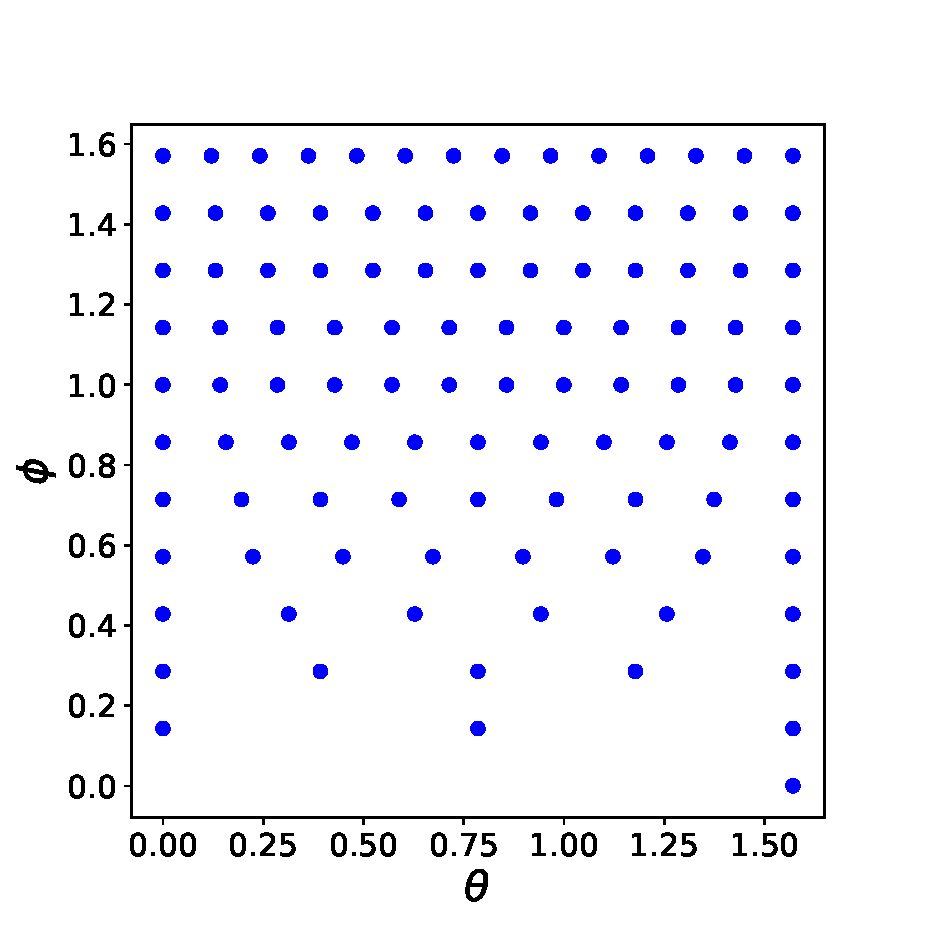
\includegraphics[width=0.3\textwidth,trim={0 0 1cm 1cm}, clip]{./fig/photos/mc_angle_space.eps}
    \label{fig:sampling}
  }
  \subfloat[\centering Locations of the simulated sources] {
    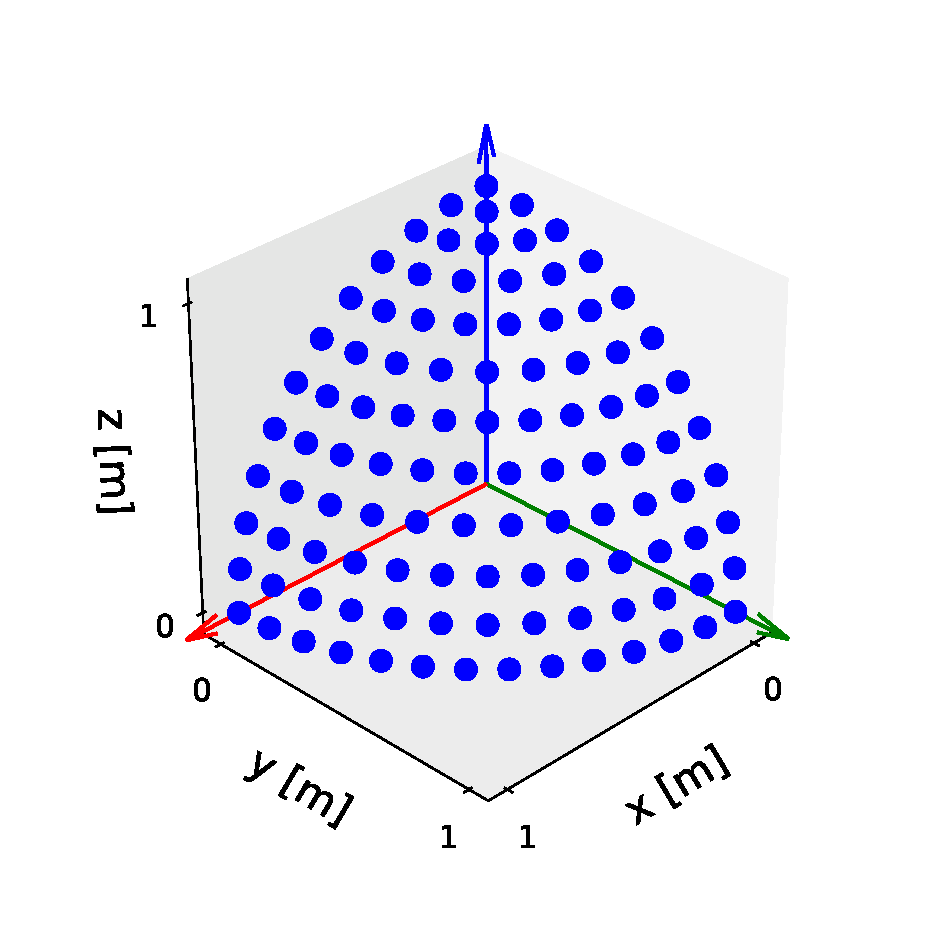
\includegraphics[width=0.3\textwidth, trim={0 0.5cm 2cm 1cm},clip]{./fig/photos/mc_sources.eps}
    \label{fig:sources_loc}
  }
  \newline
  \noindent
  \subfloat[\centering Polar coordinates] {
    \centering
    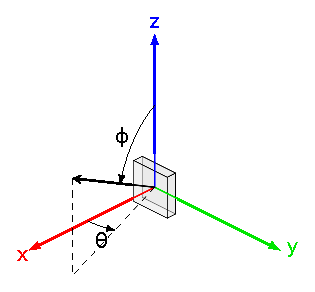
\includegraphics[width=0.25\textwidth]{./fig/photos/axes.eps}
    \label{fig:polar}
  }
  \subfloat[\centering Illustration of the solid angle definition] {
    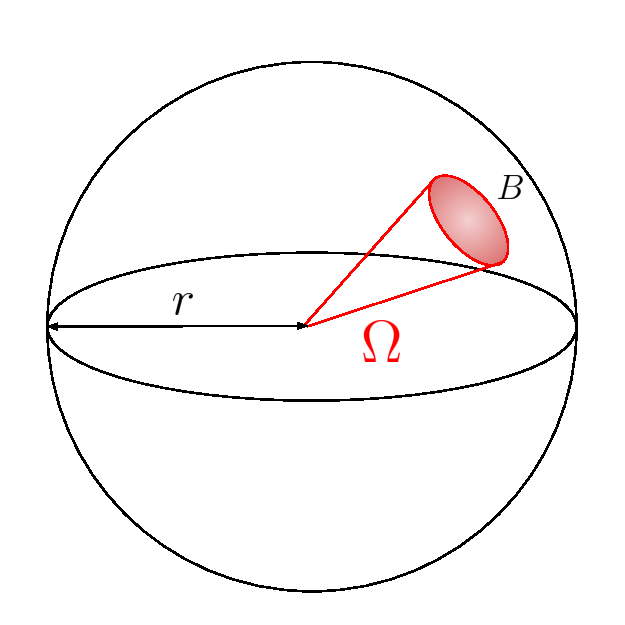
\includegraphics[width=0.25\textwidth]{./fig/photos/solid_angle_2.eps}
    \label{fig:sa}
  }
  \caption{Sampling of $\frac{1}{8}$ of the unit sphere for the Monte Carlo simulation is illustrated in \ref{fig:sampling} (angle space) and \ref{fig:sources_loc} (xyz coordinate system). 
  The polar coordinates determining the direction of incoming particle are presented in \ref{fig:polar}. 
  Finally, the solid angle definition $\Omega = \frac{B}{r^{2}}$, where $r$ is the sphere radius and $B$ is the spherical surface area, is shown in \ref{fig:sa}. }
  \label{fig:mc_multi}
\end{figure}% %%}

%%%%%%%%%%% ALGORITHM %%%%%%%%%%%%%%%%%% %%{
%%%%%%%%%%%%%%%%%%%%%%%%%%%%%%%%%%%%%%%%%%%

%\begin{algorithm}[h!]
%\caption{Monte-carlo simulation}\label{alg:cap}
  \begin{figure}
\begin{algorithmic}
\Function {create\_lookup\_table}{$N$}
  \For {$\theta \in (0, \dots ,\frac{\pi}{2})$}
    \For {$\phi \in (0, \dots , \frac{\pi}{2})$}
      \State $\mathrm{lookup\_table}(\theta, \phi) \gets \Call{compute\_probability}{\theta, \phi, N}$
    \EndFor
  \EndFor
\EndFunction
\Statex
\Function {compute\_probability}{$\theta, \phi, N$}
\State $C \gets 0$
\State $A \gets N\frac{\Omega_{\theta, \phi, d}}{4 \pi}$ \Comment{how many of $N$ particles hits the sensor}
\State $a \gets 0$
\While {$a<A$} 
  \If {\Call{is\_cone\_measured}{$\theta, \phi$}} \Comment{Compton cone measured}
  \State $C \gets C + 1 $ 
  \EndIf
  \State $a \gets a + 1$
\EndWhile
  \State \Return $C/N$ 
  \EndFunction
\Statex
  \Function{is\_cone\_measured}{$\theta,\phi$}
  \State $ray \gets \Call{sample\_sensor\_surface}{\theta,\phi}$ \Comment{ray inside the sensor after hitting its surface}
  \If{\Call{is\_Compton\_scattering}{$ray, E_{0}$}} \Comment{sample if \ac{CS} occured}
  \State $new\_ray, E_{1}, X_{1} \gets \Call{compton\_scattering}{ray, E_{0}}$ %\Comment{Sample }
  \Else{}
    \State \Return False \Comment{No Compton scattering occurred}
  \EndIf
  \If{\Call{is\_photoelectric\_effect}{$new\_ray, E_{1}$}} \Comment{Sample if \ac{PE} occurred} 
    \State $E_{2}, X_{2} \gets $\Call{photoelectric\_effect}{$new\_ray, E_{1}$}
  \Else{}
    \State \Return False
  \EndIf
  \If{\Call{passed\_outlier\_detection}{$E_{1}, E_{2}, X_{1}, X_{2}$}}  \Comment{pixel dist. and energy bounds}
    \State \Return True   
    \Else{}
    \State \Return False
  \EndIf
\EndFunction
\end{algorithmic}
      \caption{The Monte Carlo simulation pseudocode. For each $\theta, \sigma$ pair, the Monte Carlo method first computes the number of particles emitted towards the visible surface of the detector from the current position ($A$) out of all simulated particles ($N$). 
    Then a point for each of $A$ photons is randomly sampled somewhere on the visible sensor's surface, which determines the trajectory of incident photon inside the \ac{CdTe} sensor's block. 
    The Monte Carlo method counts the number of photons ($C$) that fulfilled all the following conditions: a) were emitted under the solid angle of the visible sensor's surface, 
    b) undergone the Compton scattering, 
    c) the scattered photon was absorbed, 
    d) the recorded interactions passed the outlier detection filter.
    The final probability $\frac{C}{N}$ is then stored in the lookup table.}
\label{alg:monte}
\end{figure}
%  \label{alg:monte}
%  \caption{Monte-carlo simulation}
%\end{algorithm}
%%%%%%%%%%%%%%%%%%%%%%%%%%%%%%%%%%%%%%%%%%%% %%}
\newpage
\subsection{Sensitivity computation}% %%{
The sensitivity of detection by the sensor placed at sampled position $v$ for map position $j$ is computed as:
\begin{equation}
  s_{jv} = \underset{(1-p_{air})}{\underbrace{e^{-(\mu d_{jv})} }} \underset{(p_{solid\ angle})\\(p_{compton})\\(p_{absorption})} {\underbrace{\frac{\mathrm{lookup\_table}(\phi_{jv}, \theta_{jv})}{d^{2}_{jv}}}},  
  \label{eq:sjv}
\end{equation}
where $d_{jv}$ is the Euclidean distance between map position $j$ and sensor position $v$, $\mu \approx \SI{0.01}{\meter^{-1}} $ is the linear attenuation coefficient for $\SI{622}{\kilo\electronvolt}$ photons in air, ($\phi_{jv}, \theta_{jv}$) are the polar coordinates determining the relative position of $v$ and the sensor. 
The term $\frac{1}{d^{2}_{jv}}$ in \ref{eq:sjv} ensures that the $p_{solid\ angle}$ (already contained in the $\mathrm{lookup\_table}$ for $d = \SI{1}\meter$) approximately holds even for distances other than $d = \SI{1}\meter$.

\subsubsection{Iterative formula}
The equation \ref{eq:sjv} presents the sensitivity computation for one viewpoint $v$. 
However, we would like to compute the sensitivity of detection online during the experiment for all the viewpoints previously recorded. % while keeping the memory requirements constant. 
Therefore the sensitivity vector is iteratively updated with the newly sampled viewpoints (\ac{UAV} positions).
Let denote $\mathbf{s}^{[t]}$ the sensitivity vector at time $t$.
The initial value of $\mathbf{s}^{[0]}$ is initialized with zeros. %$0$ ($s_{j}^{[0]} = 0 ,\forall s_{j}^{[0]} \in \mathbf{s}^{[0]}$).
Let us denote $V^{[t:t+1]}$ the set of viewpoints that were newly sampled between time $t$ and $t+1$ and needs to be processed. 

The sensitivity vector $\mathbf{s}^{[t+1]}$ with elements $s_{j}^{[t+1]}$ is computed as follows:
\begin{equation}
  s_{j}^{[t+1]} = s_{j}^{[t]} + \sum_{v \in V^{[t:t+1]}} s_{jv} \Delta_{v}, 
  \label{eq:sen_iter}
\end{equation}
where the sum $\sum_{v \in V^{[t:t+1]}}$ iterates over all newly processed viewpoints, 
the term $\Delta_{v} = t_{v} - t_{v-1}$ expresses the time difference between current viewpoint $v$ sampled at time $t_{v}$ and its predecessor (previous viewpoint generated from the trajectory of the same \ac{UAV}) sampled at time $t_{v-1}$. 

This formulation of sensitivity has multiple advantages.
Firstly, the memory requirements for storing the vector $\mathbf{S}$ remain the same during the whole experiment. The values $s_{j}$ are updated in place.
Secondly, the sensitivity is updated online as new sampled trajectories of the \ac{UAV} arrive. Therefore the computation time scales well with the increasing duration of the experiment.
Lastly, it takes into account the time difference between sampled viewpoints $\Delta_{v}$.% %%}

%%%%%%%%%%%%%%%%%%%%%%%%%%
%%%%%%%%%%%%%%%%%%%%%%%%%%
%%%%%%%%%%%%%%%%%%%%%%%%%%
\section{System matrix}
\label{sec:system}
The system matrix $\mathbf{T} \in \mathbb{R}^{I \times J}$ is defined as
\begin{equation}
t_{ij} =  P(\textrm{detected in } i | \textrm{emitted from } j).
\end{equation}
In other words, it says how likely the photon causing measurement $i$ came from the map position $j$.
The illustration of the system matrix is depicted in figure \ref{fig:sys_ilustration}, where the blue colour represents $t_{ij}$ values of the individual cells. 
\begin{figure}[!h]
  \centering
    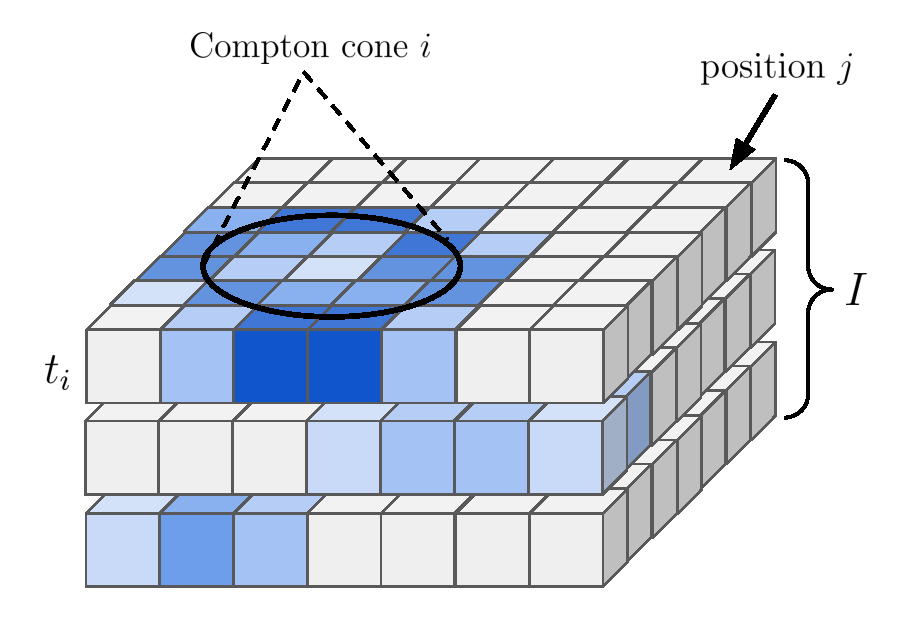
\includegraphics[width=0.48\textwidth]{./fig/photos/systemmmm.eps}
  \caption{System matrix $\mathbf{T}$. The blue colour represents the value of $t_{ij}$ in each cell.}
    \label{fig:sys_ilustration}
\end{figure}

%The main question remains the same as for the sensitivity computation: how to evaluate the system matrix for a given scenario and \ac{pix} sensor?

The measurement $i$ is composed of multiple components:
\begin{equation}
  i_{full} = (\beta_{i}, v_{i}, a_{i}, X_{1}, E_{1}, X_{2}, E_{2}),
\end{equation}
where:
\begin{itemize}
  \item $\beta_{i}$ is the reconstructed Compton angle,
  \item $v_{i}$ is the 3D pose (position and orientation) of the sensor in world coordinates at the time when the event was recorded,
  \item $\mathbf{a}_{i}$ is the axis vector of the reconstructed Compton cone,
  \item $X_{1}$ is the position of the first interaction (Compton scattering) inside the detector,
  \item $E_{1}$ is the measured energy of the electron that was created as a side product of the Compton scattering,
  \item $X_{2}$ is the position of the second interaction (absorption) inside the detector,
  \item $E_{2}$ is the measured energy of the absorbed electron.
\end{itemize}
%The first interaction (electron produced as a side product of \ac{CS}) at position ${X_{1}}$ with measured energy $E_{1}$) 
%and the second interaction (absorbed electron at position $X_{2}$ inside the sensor with measured energy $E_{2}$).
%The Compton cone $i$ with scattering angle $\beta_{i}$ is then reconstructed from these measurements using equation \ref{eq:theta}.
%The position of the sensor at the time when the Compton effect was measured is denoted $v_{i}$ (and is composed of position and orientation in the world coordinates).

\subsection{Probabilistic description}
A series of random occurrences should happen for a photon emitted at position $j$ with initial energy $E_{0}$ to be detected by the Compton camera as measurement $i$.
The term $t_{ij}$ can be described with probabilities as:
\begin{itemize}
  \item $p_{solid\ angle}(j, v_{i}) $: the probability that the photon is emitted at position $j$ under the right solid angle towards the visible surface of the detector at position $v_{i}$,
  \item $(1-p_{air}(d_{jv_{i}}))$: the probability that the photon reaches the detector surface (not being absorbed along the way, where $d_{jv_{i}}$ is the distance from $j$ to detector pose $v_{i}$),
  \item $\bar{p}_{compton}(j, X_{1}, E_{0}, \beta_{i})$: the probability that it interacts with the matter of the detector at position $X_{1}$ and undergo Compton scattering under angle $\beta_{i}$ while losing energy $E_{1}$ to the electron that is immediately measured by the detector,
  \item $\bar{p}_{absorption}(X_{1}, X_{2}, E_{0}, E_{1})$: the probability that the scattered photon interacts with the matter of the detector at position $X_{2}$, is absorbed and energy $E_{2}$ is measured by the detector during the absorption.
\end{itemize}
Same as in the sensitivity section, the presented model is simplified, and several assumptions are made. 
It is assumed that the first interaction is a Compton scattering and the second interaction is the photoelectric effect (absorption) (which might not always be true since other interactions might occur), it is assumed that $E_{0} = E_{1} + E_{2}$, etc.
Unlike in sensitivity computation (where $s_{j}$ describes the probability that a photon emitted from $j$ is detected anywhere by the detectors), the elements of system matrix $t_{ij}$ describe the probability that a photon emitted from $j$ was recorded in measurement $i$, therefore $p_{compton}\neq \bar{p}_{compton}$ and  $p_{absorption}\neq \bar{p}_{absorption}$.

\subsection{Inspiration from literature}
The nuclear medicine literature provides multiple models for the system matrix, such as \cite{wilderman}. 
However, the model is designed for two-layer Compton camera and for scenarios where the detector size is relatively large compared to the distance to the source. Therefore, the geometry of the Compton camera must be considered.
Work presented in \cite{maxim2016} described a simplified model for the Compton camera, which size is negligible compared to the distance to the source of radiation (for two-layer Compton camera).
The energy measurement uncertainties are approximated using Gaussian distribution.
Both of these models do not take into account the effect of environmental attenuation.
Despite all of these differences, it served as an inspiration for the proposed approach.

\subsection{Simplifications of the problem}
Efficient evaluation of $\bar{p}_{compton}$ and $\bar{p}_{absorption}$ is challenging since it depends on the length of the incoming and scattered ray inside the detector.
In the given scenario, the size of the \ac{pix} detector is negligible ($14 \times 14 \times 2 \ \mathrm{mm}$) compared to the distance between the detector mounted on the \ac{UAV} (flying at least $\SI{3}\meter$ above the ground) and source of radiation.
Because of that, modelling $p_{solid\ angle}$ (probability that the particle reaches the detector) and $p_{air}$ (air attenuation) is relatively more important than the accurate modelling of probabilities of events inside the detector.

The following simplification is made:
The measurement $i$ is represented as
\begin{equation}
  i = (\beta_{i}, v_{i}, a_{i})
\end{equation}
and the measured energies and exact positions of interactions inside the detector are ignored,
the Compton camera detector is approximated as a single point with position and orientation $v_{i}$.
However, the probability of detecting the Compton effect produced by particles incoming from some direction is not uniform for all directions (given the non-uniform shape of the sensor).
The lookup table from the previous section (representing the chance that a particle incoming from a specific direction cause any detectable Compton effect, not just the one measured in $i$) is used to approximate the direction sensitivity of the detector.

\subsection{System matrix computation}
The elements $t_{ij}$ of system matrix $\mathbf{T}$ are computed as:
\begin{equation}
  t_{ij} = \underset{(1-p_{air})}{\underbrace{e^{-(\mu d_{jv_{i}})}}}\ 
  \underset{\bar{p}_{compton}} {  \underbrace{K(\beta_{i}, E_{0})\ h(\delta_{ij}|\sigma, \alpha_{ij})}} \
  \underset{(p_{solid\ angle})\\(p_{compton})\\(p_{absorption})} {\underbrace{\frac{\mathrm{lookup\_table}(\phi_{jv}, \theta_{jv})}{d_{jv_{i}}^{2}}}}
  ,%s_{jv} = \underset{(1-p_{air})}{\underbrace{e^{-((\mu/\rho) d_{jv})} }} \underset{(p_{solid\ angle})\\(p_{compton})\\(p_{absorption})} {\underbrace{\frac{\mathrm{lookup\_table}(\phi_{jv}, \theta_{jv})}{d^{2}_{jv}}}},  
  \label{eq:system_matrix_full}
\end{equation}
where:
\begin{itemize}
 \item $d_{jv_{i}}$ is the Euclidean distance between the map position $j$ and sensor position $v_{i}$, 
\item $\mu \approx \SI{0.01}{\meter^{-1}} $ is the linear attenuation coefficient for $\SI{622}{\kilo\electronvolt}$ photons in air\item $K(\beta_{i}, E_{0})$ is the Klein-Nishina formula representing the probability of Compton scattering under estimated angle $\beta_{i}$ for an incoming particle with energy $E_{0}$,
\item $h(\delta_{ij}|\sigma_{j})$ is a Gaussian kernel (the ``blurring factor'') representing the uncertainty in angle measurement,
\item $\delta_{ij}$ is angle difference $|\beta_{i}-\beta_{j}|$, where $\beta_{j}$ is the angle between cone axis vector $a_{i}$ and vector $|j-v_{i}|$, 
\item $\sigma$ is standard deviation and $\alpha$ is the minimal angle difference due to discretization noise,
\item $\mathrm{lookup\_table}(\phi_{jv}, \theta_{jv})$ is the lookup table defined in section \ref{sec:sensitivity}.
\end{itemize}

The angular difference $\delta_{ij}$ in equation \ref{eq:system_matrix_full} comprise the measured Compton cone.
If the reconstructed Compton cone (with origin $v_{i}$, axis vector $a_{i}$ and Compton angle $\beta_{i}$) would perfectly intersect the map position $j$, then the angular difference would be $\delta_{ij} = 0$, as illustrated in figure \ref{fig:system_comp}.
However, this holds only for a perfect world without noise.

\begin{figure}[!h]
  \centering
    \includegraphics[width=0.4\textwidth]{./fig/photos/system_comp.eps}
    \caption{An illustration of the measurement $i$, which is composed of cone origin $v_{i}$, axis vector $a_{i}$ and Compton angle $\beta_{i}$.}
    \label{fig:system_comp}
\end{figure}
\subsubsection{Measurement noise}
The real-world measurements are affected by measurement noise. Hence the reconstructed cone might not intersect the real position of emission.
The measurement noise might be present in the measured energies $E_{1}$ and $E_{2}$ (that are affecting the Compton angle $\beta_{i}$ , see equation \ref{eq:compton_beta_formula}) 
as well as in the positions of interactions inside the detector ($X_{1}$ and $X_{2}$) 
that are affecting the cone axis $a_{i}$.
The influence of noise in energy measurement (Compton angle $\beta$) is modelled using Gaussian function with ``standard deviation'' $\sigma$:
\begin{equation}
  h(\delta_{ij}|\sigma) = e^{-\frac{1}{2}(\frac{\delta_{ij}}{\sigma})^{2}}.
  \label{eq:gau}
\end{equation}
If the angle difference is large ($\delta_{ij}<3\sigma$), then we set $h(\delta_{ij}|\sigma) = 0$.
The important question is how to set the parameter $\sigma$, that is influencing the width of the function \ref{eq:gau}.
The datasheet\footnote{Available at: https://advacam.com/camera/minipix-tpx3}
states that the energy resolution of used Timepix3 pixel detector is $4.5$--$9.9\ \mathrm{kEV}$. 
The dependence of angular uncertainties on the energy resolution of two-layer Compton cameras was studied in \cite{ordonez}.
The measurement of the energies is not the only source of noise in the detection pipeline.
The $h(\delta_{ij}|\sigma)$ function should disperse the conical back-projections in order to tackle other inaccuracies, such as noise in the sensor's position or wrongly estimated axis of the Compton cone. 
The exact estimation of angular uncertainty (and other sources of noise) is beyond the scope of this thesis.
%Other sources of noise (such as positions of interaction inside the detector $X_{1}$, $X_{2}$, especially depth of interaction in the sensor block) are difficult to model as well.
For ``proof of concept'' demonstration, the value $\sigma$ was set empirically based on recorded data from experiments with real \ac{pix} sensors.

\subsubsection{Discretization error}
Another possible source of noise is the discretization of the area of interest, which is divided into $J$ discrete bins (each represented by its centre position) with resolution $r$.
Even perfectly measured and reconstructed Compton cone might not intersect the real position of emission (meaning $\delta_{ij}$ would be non-zero) due to the discretization of $J$.
Let us define maximal error for measurement $i$ and position $j$ caused by discretization as
\begin{equation}
  \alpha_{ij} = \mathrm{arctan}(\frac{x}{d_{jv_{i}}}),
  \label{eq:alpha}
\end{equation}
where $d_{jv_{i}}$ is the distance between cone origin at position $v_{i}$ and map position $j$ and $x$ is the maximal allowed distance between projected cone and discrete position $j$, $x = l$.
The situation is illustrated in figure \ref{fig:discret}.
\begin{figure}
  \centering
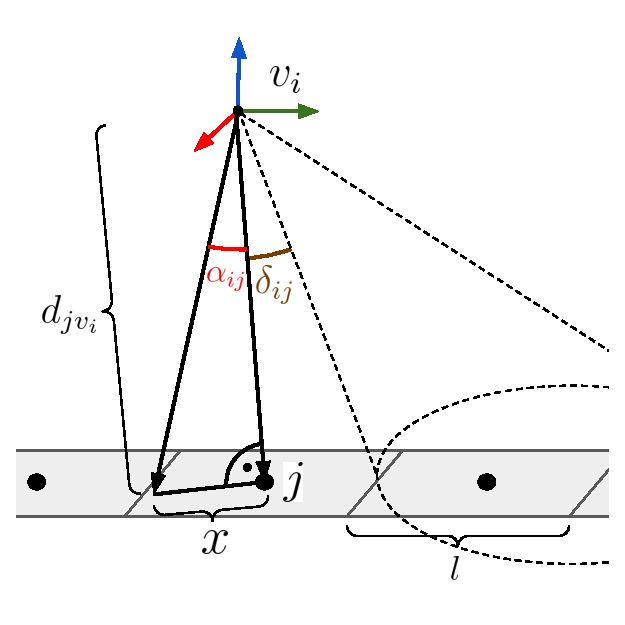
\includegraphics[width=0.4\textwidth]{./fig/photos/discret.eps}
  \caption{ 
Illustration of discretization error. The maximal angle difference caused by discretization error $\alpha_{ij}$ is computed for each map position $j$.}
  \label{fig:discret}
\end{figure}
Taking into account the discretization as well as measurement noise, the term $h(\delta_{ij}|\sigma, \alpha_{ij})$ in equation \ref{eq:system_matrix_full} which is projecting the cone to the map positions is defined as
\begin{equation}
h(\delta_{ij}|\sigma) =
\begin{cases}
1 & \text{if $\delta_{ij}\leq \alpha_{ij}$}\\ 
e^{- \frac{1}{2}(\frac{\delta_{ij}}{\sigma})^{2}} & \text{if $\delta_{ij} > \alpha_{ij}$ and  $\delta_{ij} \leq 3\sigma_{j}$} \\
0 & \text{otherwise}
\end{cases}, 
\end{equation}
where $\alpha_{ij}$ is the maximal angle difference caused by discretization error defined in equation \ref{eq:alpha}.








































%%%%%%%%%%%%%%%%%
%%%%%%%%%%%%%%%%%%%%
%%%%%%%%%%%%%%%%%%%%%
%%%%%%%%%%%%%%%%%%%%
%%%%%%%%%%%%%%%%
%%%%%%%%
%%%%%%%%%%
%%%%%%%%%%
%%%%%%%%%%%%
%%%%%%%%%%%%%%
%%%%%%%%%%%%
%


%!TEX root = ../main.tex

\chapter{Multirobot search strategy}

This chapter presents a multirobot search strategy for a group of \ac{UAV}s equipped with Compton camera for online estimation of sources of ionizing radiation, which is based on the \ac{MLEM} method described in the previous chapter.
First part describes the objectives and requirements for such method.
The whole system is described in the next section, as well as individual components of the system.
\section{Objectives}
%The \ac{MLEM} method proposed in the previous chapter provides the maximum likelihood estimate of the measured data.
%When the number of detected Compton events is low, the maximum likelihood estimation method might suffer of inaccurate 

\subsection{Measure as much data as possible}
As stated before, the emission of $\gamma$ particles as well as the detection of Compton events are stochastic processes.
The intensity of radioactive emission follows the inverse square law, which means that it decreases as the distance from the source increases.
Due to the small size of the detector, large distances between \ac{UAV}s and sources of ionizing radiation, and the fact that only $2\%$ of $\gamma$ particles reaching the detector are detected by the Compton camera (on average), the number of detected events is limited.
The accuracy of the \ac{MLE} method depends on the number of detected Compton events.
If the number of detected cones is low, the \ac{MLE} method might converge to false detections since the particle could originate from any position on the surface of the Compton cone.
To accurately localize the sources of ionizing radiation, the \ac{UAV}s should collect as many measurements as possible.
This requires the \ac{UAV}s to fly as close as possible to the currently most likely source estimates to either confirm or disprove the presence of the radioactive source at the given position.
It is also desired that the drones stay in motion (instead of hovering above the points of interest), since measurements from different angles are beneficial for sources localization.

\mycomment{% %%{
  As stated before, the emission as well as the detection of Compton events are stochastic processes.
  The intensity of radioactive emission decreases with inverse square law as the distance from source grows.
  Because of the small size of the detector, large distances between \ac{UAV}s and sources oinizing radiation and the fact that only $2 \%$ of $\gamma$ particles that reach the detector are detected by the Compton camera, the number of detected events is limited.
  The accuracy of \ac{MLE} method from definition depends on the number of detected Compton events.
  When the number of detected cones is low, the \ac{MLE} method might converge to false detections (since the particle could originated from any position on the surface of Comtpon cone).
  To measure more data, the \ac{UAV}s should collect as many measurements as possible.
  It requires the \ac{UAV}s to fly as close as possible to the currently most likely source estimates to either confirm or disprove the presence of the radioactive source at the given position.
}% %%}

\subsection{Search for unobserved sources of ionizing radiation}
The sensitivity vector $\mathbf{S}$ described in the previous chapter provides information about coverage of each discrete point $j$ in the area of interest.
The autonomous \ac{UAV}s should control their motion in the way that the whole area is covered.
In another words, the minimum value of sensitivity $\mathrm{min}(s_{j})$ among all positions in the search space should be as high as possible to increase the chance of observing sources that were not yet detected.

\subsection{Active search strategy}
There are two general strategies how an area of interest can be explored by a group of autonomous \ac{UAV}s in order to measure data and estimate sources of ionizing radiation - offline and online.
In offline search, the \ac{UAV}s typically follow predefined paths and collect measurements, that are processed all at once after the flight. 
In online search, the estimation process is performed online and the \ac{UAV}s may react accordingly to the current output of the radiation mapping method.
Incorporating the output of the mapping method into the feedback control loop 
might lead to better estimate (since more measurements might be acquired) and fasten the search time.
In general, an active search strategy allows the group of \ac{UAV}s to use its full potential, therefore it is desired for the given task.

\mycomment{% %%{
\subsection{Motivation for mlem}
Neco o tom yze i negativni mereni jsou dulezity
  The emission of $\gamma$ particles as well as the detection of Compton events are stochastic processes.
  Only a small fraction of emitted $\gamma$ particles are detected by the small \ac{pix} sensor located several meters from the radioactive source.
  Moreover, the intensity of radioactive emission decreases with the inverse square law as the distance from the source grows.
  Taking into account also ther properties of the ionizing radiation and the detection process, the acquired measurements are highly dependent on the trajectories of the \ac{UAV}s performing the search mission.
  The \ac{UAV}s might be controlled in two ways: they can either a) follow some trajectory that cover the whole area of interest uniformly or b) the trajectory of the \ac{UAV} is arbitrary and the coverage of the space is not uniform.
  However, it doesn't use the whole potential of small and agile \ac{UAV}s carrying the Compton camera.
  In b) approach, it is required 
}% %%}

\mycomment{% %%{
  \subsection{Centralized vs. decentralized}
  The multirobot systems can be classified into two groups: centralized and decentralized.
  In a centralized approach, a central control unit is responsible for coordinating the actions of all the robots in the network. 
  This centralized system can provide global information to each robot, enabling them to make more informed decisions based on the overall state of the system.
  On the other hand, it is vulnerable to single points of failure and it requires reliable communication between each agent and the central unit.
  In decentralized system, each robot operates independently, making decisions based on local information and communication with other robots in the network. 
  This approach can provide increased fault tolerance and can be more adaptable to changing conditions. 
  However, the lack of a central control unit can make it challenging to ensure that all robots are efficiently working towards a common goal.
}% %%}

\section{System design description}
\subsection{Task specification}
The proposed search strategy is based on the objectives described above - the group of \ac{UAV}s should autonomously explore the area of interest with no previous knowledge about number, activity or position of sources of ionizing radiation and localize such sources as fast as possible.
The operation of the \ac{UAV}s is divided into two main tasks:
\begin{itemize}
  \item \textbf{exploration} - the drones should explore the area of interest and increase the chance that none of the sources of $\gamma$ particles would be unobserved,
  \item \textbf{exploitation} - the drones should exploit positions where \ac{MLEM} mapping method estimated some emission activity to either confirm the hypothesis and collect more measurements or disprove it (=increase accuracy of the estimation).
\end{itemize}

%\subsection{Assumptions}
%It is assumed that 
%a) a communication via wireless network is provided, 
%b) the mission is performed in outdoor environment with no obstacles, 
%c) the sources of ionizing radiation are located somewhere on the ground, that is for simplicity assumed to be a flat plane.

\subsection{Multirobot architecture}
The multirobot systems can be classified into two groups: centralized and decentralized.
In a centralized approach, a central control unit is responsible for coordinating the actions of all the robots in the network. 
This centralized system can provide global information to each robot, enabling them to make more informed decisions based on the overall state of the system.
%On the other hand, it is vulnerable to single points of failure and it requires reliable communication between each agent and the central unit.
In decentralized system, each robot operates independently, making decisions based on local information and communication with other robots in the network. 

\begin{figure}[!htb]
    \centering
    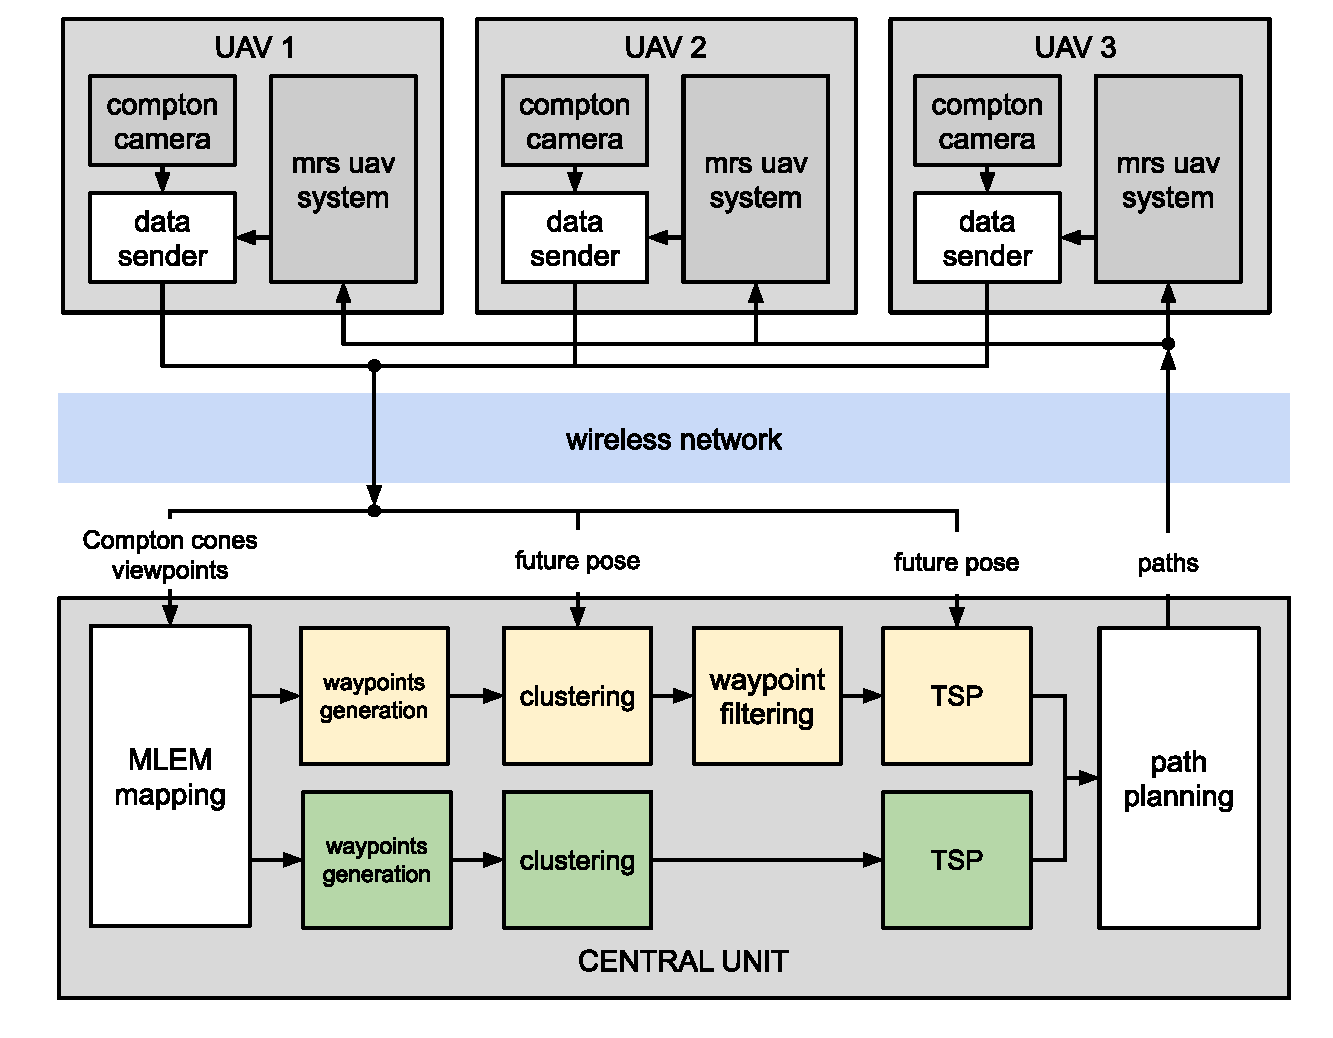
\includegraphics[width=0.99\textwidth]{./fig/photos/system_new.eps}
    \caption{\centering The system architecture diagram. The search and planning method is composed of \ac{MLEM} radiation mapping node, waypoint generation, clustering, waypoint filtering, optimal sequence deduction using TSP and path planning. The exploration (green) and exploitation (yellow) waypoints are processed separately.}
    \label{fig:sysarch}
\end{figure}

The centralized multirobot architecture is used in this project.
The visualization of the system can be seen in figure \ref{fig:pipeline}.
The \ac{UAV}s are communicating via wireless \ac{Wifi} network.
The amount of information shareable via such network is limited.
Therefore all the \ac{MLEM} computations and running on a ground station and the \ac{UAV}s and ground station share the minimal amount of information possible.
All the \ac{UAV}s send its current position and future position in $\SI{2}\second$ as a custom \ac{ROS} message (with frequency $\SI{2}\hertz$), 
together with all newly measured Compton cones.
The ground station processes the measurements and command the \ac{UAV}s by sending non-colliding path for each of them via the wireless network.
The centralized approach have several advantages in this scenario:
The \ac{MLEM} estimate is computed at once, not requiring to share or merge the map with other \ac{UAV}s via the wireless network or run the estimation onboard each drone separately.
The centralized task allocation and path planning is much more straightforward compared to the decentralized approach, where the agents would need to negotiate between each other..
This design choice of course have some disadvantages as well.
The centralized system is vulnerable to single point of failure and the communication between the ground station and all \ac{UAV}s must provided. 

\subsection{Custom data message}
A custom \ac{ROS} message was developed to transfer necessary data from \ac{UAV} to the ground station.
The message consists of the \ac{ROS} header containing the coordinate frame (all drones share the same coordinate system given their gps origin),
timestamp specifying the time when it was created,
pose of the drone and its Compton camera 
and predicted point representing the future position of the \ac{UAV} in time horizon of $2$ seconds (which is generated by the \verb|mpc tracker| that is part of the mrs uav system \cite{mrs_system}).
The structure of the message is shown here:

\begin{lstlisting}[caption={DroneDataMsg.msg (caption)}, title={Custom message for data sharing between \ac{UAV} and central unit.}, label={code1}]
Header header
geometry_msgs/Pose pose
geometry_msgs/Pose sensor_pose
geometry_msgs/PointStamped predicted_point
std_msgs/String status
\end{lstlisting}


\section{Search and planning strategy description}
The central node responsible for search and planning strategy is composed of multiple parts.
The main steps are depicted in figure \ref{fig:sysarch}.

% FIGURES STEPS of PIPELINE
\begin{figure}[!htb]% %%{

  \subfloat[\centering \textbf{waypoint generation} - detected local maxima of \ac{MLEM} estimate] {
    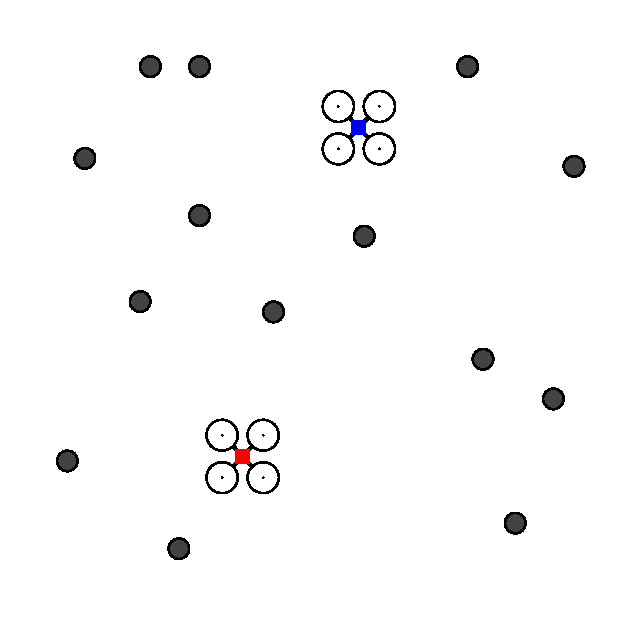
\includegraphics[width=0.3\textwidth]{./fig/photos/pip1.eps}

    \label{fig:pip1}
  }
  \subfloat[\centering \textbf{waypoint generation} - weighing and filtering] {
    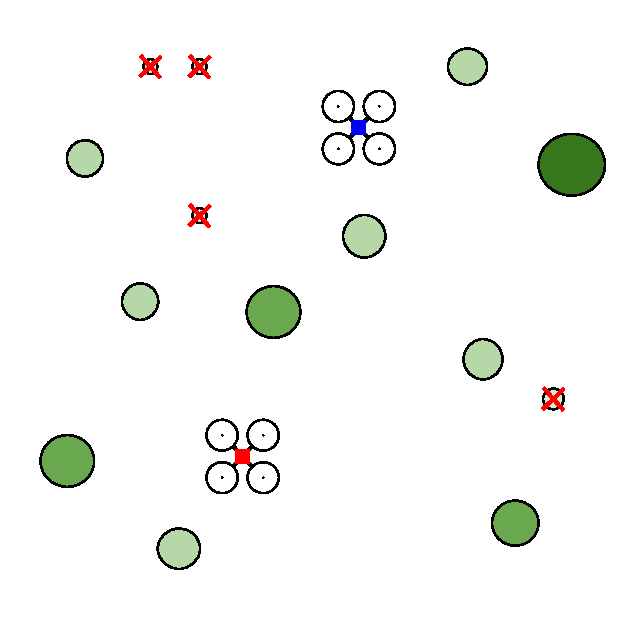
\includegraphics[width=0.3\textwidth]{./fig/photos/pip2.eps}
    \label{fig:pip2}
  }
  \subfloat[\centering \textbf{clustering} - assigning waypoints to \ac{UAV}s] {
    \includegraphics[width=0.3\textwidth]{./fig/photos/pip3.eps}
    \label{fig:pip3}
  }
  \newline
  \subfloat[\centering \textbf{waypoint filtering} - removal of recently visited waypoints based on short-term sensitivity] {
    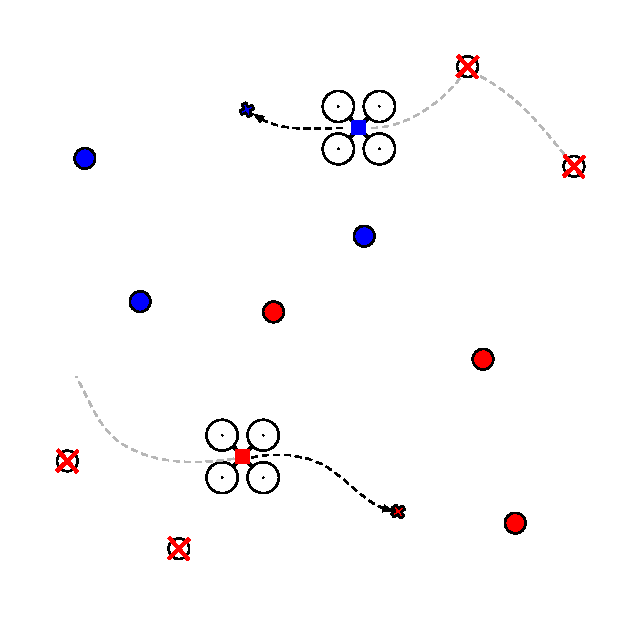
\includegraphics[width=0.3\textwidth]{./fig/photos/pip4.eps}
    \label{fig:pip4}
  }
  \subfloat[\centering \textbf{TSP} - optimal sequence determination] {
    \includegraphics[width=0.3\textwidth]{./fig/photos/pip5.eps}
    \label{fig:pip5}
  }
  \subfloat[\centering \textbf{path planning} - find non-colliding paths connecting the waypoints] {
    \includegraphics[width=0.3\textwidth]{./fig/photos/pip6.eps}
    \label{fig:pip6}
  }
  \caption{Individual steps of the system architecture.}
  \label{fig:pipeline}
\end{figure}% %%}

In the beginning, the exploitation waypoints are generated from the current \ac{MLEM} estimate (figure \ref{fig:pip1}).
Each waypoint is assigned a weight and only subset of waypoints with highest weights are processed to the next step (figure \ref{fig:pip2}).
The waypoints are assigned to the \ac{UAV}s using clustering method (figure \ref{fig:pip3}).
The recently visited exploitation waypoints are removed in the next step (figure \ref{fig:pip4}).
All points are connected into an optimal sequence (starting at the future position of the drone) using TSP (figure \ref{fig:pip5}).
Finally, non-colliding paths are planned for all \ac{UAV}s (figure \ref{fig:pip6}).
The more detailed description of each individual step follows in the next sections.


\mycomment{% %%{
  \section{multirobot approach}
  The previous chapter presented the method for localizing sources of ionizing radiation.
  %Given the collected measurements, it can compute the maximum likelihood estimate of the sources locations.
  Moreover, the sensitivity computed in the \ac{MLEM} method provides information about how much has been the area explored by the compton cameras onboard the \ac{UAV}s.

  This motivates the search strategy described in this section:
  The movement of the \ac{UAV}s should be controlled in a way that they simultaneously perform the following tasks:
  \begin{itemize}
    \item \textbf{exploration} - explore the least explored maps in the area of interest and increase the chance that so far unobserved sources of radiation will be detected
    \item \textbf{exploitation} - fly where the radioactive sources are likely present (based on the current maximum likelihood estimate) to improve the accuracy of the estimate. 
  \end{itemize}

%The maximum likelihood approach requires collecting as many measurements as possible to make the estimate more accurate.
%At the same time, the drones should explore the unexplored area to increase chance that the estimation method won't miss any source of ionizing radiation.
%The task for the mutirobotic system can be summarized as follows:
%\begin{itemize}
%  \item \textbf{exploration} - explore the least explored maps in the area of interest
%  \item \textbf{exploitation} - acquire more measurements from areas, where the source of ionizing radiation is likely present
%\end{itemize}
}% %%}





%%%%%%%%%%%%%%%%%%%%%%%%%%%%%%%%%
%%%%% WAYPOINTS GENERATION %%%%%%
%%%%%%%%%%%%%%%%%%%%%%%%%%%%%%%%%


\section{Waypoints generation}% %%{
\subsection{Exploitation}
\subsubsection{Local maxima filter}
The current estimate of ionizing radiation sources positions serves as an input for the waypoint generation method.
The map estimated by the \ac{MLEM} method is processed and local maxima of the map are detected.
Local maximum is a cell in the discretized map that has the highest value among all cells in its neighborhood. 
The size of the sliding window determining the neighborhood of each cell is a parameter that can be set.
The local maxima filter is illustrated in figure \ref{fig:filter}.

%figure filter%%{
\begin{figure}[!htb]
  \centering
  \subfloat[\centering input of the filter] {
    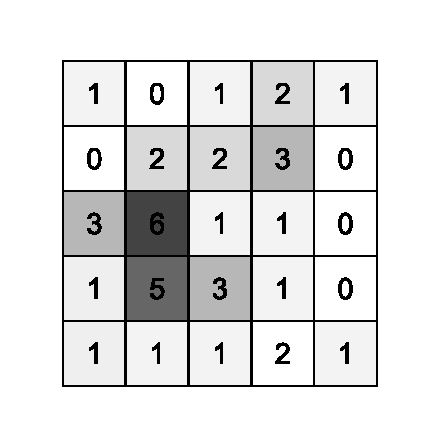
\includegraphics[width=0.2\textwidth]{./fig/photos/filter1.eps}

    \label{fig:fil1}
  }
  \subfloat[\centering filter window size 3] {
    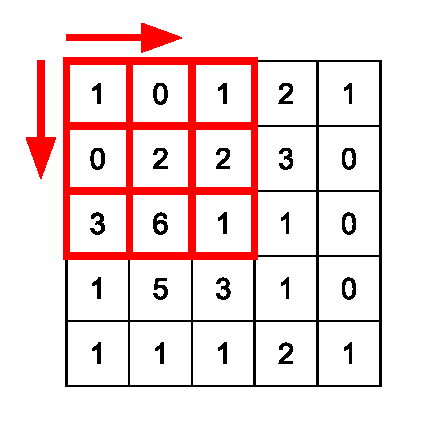
\includegraphics[width=0.2\textwidth]{./fig/photos/filter3.eps}
    \label{fig:fil2}
  }
  \subfloat[\centering detected local maxima] {
    \includegraphics[width=0.2\textwidth]{./fig/photos/filter2.eps}
    \label{fig:fil3}
  }
  \caption{Local maxima filter demonstration}
  \label{fig:filter}
\end{figure}% %%}

\subsubsection{Waypoint weighting and filtration}
The waypoints associated with local maxima are weighted using following formula:
\begin{equation}
  w_{j_{weight}} = \frac{\lambda_{j}}{    s_{j_{normalized}} },
\end{equation}
where $s_{j_{normalized}} = \frac{ s_{j} }{ \underset{j}{\mathrm{max}}(s_{j})}$ is a sensitivity value normalized to range $[0, 1]$.
The purpose of the weighting step is following: it should prioritize the waypoints (local maxima) that are less explored (the sensitivity value is small compared to other waypoints).
The list of possible waypoints is then sorted from the highest $w_{j_{weight}}$ to the lowest.
Top $n$ waypoints based on the $w_{j_{weight}}$ are propagated further in the algorithm, the rest is ignored (parameter $n$ is set to $n = 10d$, where $d$ is number of drones used for exploitation).
The aim of filtering step is to remove the local maxima that were caused by noise in the \ac{MLEM} estimation.% %%}

\subsection{Exploration}
The task is to explore the map positions that have low sensitivity values (the probability that particle emitted from such position to be detected is low).
The process of generating waypoints for exploration is illustrated in figure \ref{fig:downsampling}.
The sensitivity vector $\mathbf{S}$ is downsampled by a mean filter with the stride equal to the filter window size.
The positions in the downsampled map are then sorted based on the mean sensitivity value.
Arbitrary percentage $p$ of the map poses with lowest sensitivity values is taken and exploration waypoints are generated in the centers of such downsampled map positions, as shown in figure \ref{fig:down3} for $p = 25\%$.

%figure downsampling%%{
\begin{figure}[!htb]
  \centering
  \subfloat[\centering input vector $\mathbf{S}$ in 2D] {
    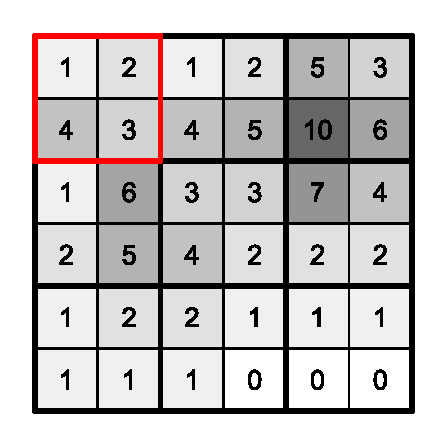
\includegraphics[width=0.25\textwidth]{./fig/photos/downsampling1.eps}

    \label{fig:down1}
  }
  \subfloat[\centering downsampled map (for window size and stride both equal 2)] {
    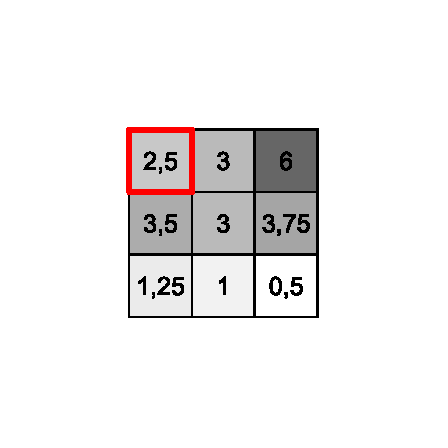
\includegraphics[width=0.25\textwidth]{./fig/photos/downsampling2.eps}
    \label{fig:down2}
  }
  \subfloat[\centering generated waypoints in the downsampled map for $p = 25\%$] {
    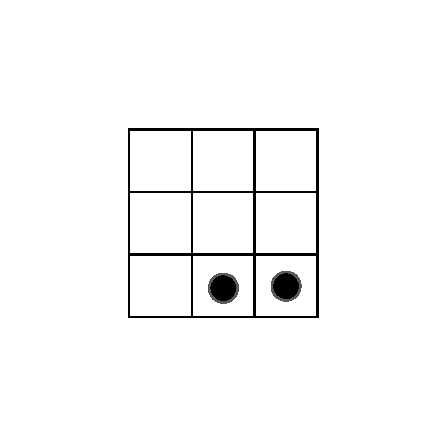
\includegraphics[width=0.25\textwidth]{./fig/photos/downsampling3.eps}
    \label{fig:down3}
  }
  \caption{Downsampling and waypoint generation process for exploration}
  \label{fig:downsampling}
\end{figure}% %%}


%%%%%%%%%%%%%%%%%%%%%%%
%%%%% CLUSTERING %%%%%%
%%%%%%%%%%%%%%%%%%%%%%%
\section{Clustering}% %%{
Clustering belongs to the group of unsupervised machine learning methods.
The goal of clustering is to partition the data into distinct groups (clusters), where data points within the same cluster are more similar to each other than to those in other clusters.
The euclidean distance is the measure of similarity used in this scenario.
The clustering algorithm of choice for the given task is \textbf{KMeans}, originally described in \cite{kmeans}.
The generated and filtered waypoints need to be assigned to the individual \ac{UAV}s. 
First step for that is clustering into groups, one group for each \ac{UAV} contributing to exploitation.

\subsection{KMeans algorithm}
The basic euclidean version of KMeans is defined as follows:
Let's denote data points to be clustered as $\{\mathbf{w}_{1}, \mathbf{w}_{2}, \dots , \mathbf{w}_{n}\}$.
The task is to assign each of the data points into one of the $k$ clusters, $\{C_{1}, C_{2}, \dots, C_{k}\}$.
Each cluster is represented by its centroid, $\mathbf{c}_{1}, \mathbf{c}_{2}, \dots, \mathbf{c}_{k}$.
The criterion function that should be minimized is then formulated as
\begin{equation}
  J = \sum_{i = 1}^{k} \sum_{\mathbf{w} \in C_{i}} \| \mathbf{w} - \mathbf{c}_{i} \|^{2}.
\end{equation}
In other words, we want to find such clusters so that the sum of distances between data points and corresponding centroids of clusters will be minimal.
\textbf{KMeans} is an iterative algorithm.
In each iteration, it assigns each data point to the nearest centroid based on the euclidean distance. 
After all data points are assigned to clusters, the centroids are updated by calculating the mean of all data points in each cluster. 
These two steps are repeated until convergence.
It is important to note that the outcome of the algorithm depends on the initialization of centroids and the method converge to local minima based on that initialization.

\subsection{Constrained KMeans and initialization}
For the purpose of assigning waypoints to the \ac{UAV}s, the optimality of the solution is not required.
However, we would like to assign waypoints to the \ac{UAV} that are in its neighborhood.
Moreover, we would like to guarantee that each \ac{UAV} has at least one point assigned (the standard version of KMeans does not guarantee non-emptiness of the clusters).
Therefore the constrained variant of KMeans \cite{constrained_kmeans} is used already implemented in \verb|k-means-constrained|\footnote{Available at: https://pypi.org/project/k-means-constrained/} python package.
The centroids are initialized at the future positions of the \ac{UAV}s.
The minimum number of waypoints in each cluster is set to $2$ (if the number of waypoints is large enough).% %%}

%%%%%%%%%%%%%%%%%%%%%%%
%%% FILTERING RECENT %%%
%%%%%%%%%%%%%%%%%%%%%%%
\section{Filtering recently visited waypoints}% %%{
The following assumption is made:
to acquire more measurements from different sides and localize the sources more precisely, it is better to keep the \ac{UAV}s in motion rather then statically hover at certain position for longer time.
No waypoint should be left unexplored for longer time.
Therefore are prioritized the waypoints that were not recently explored by any of the \ac{UAV}s (meaning that no \ac{UAV} was in a close proximity of the sensor in past seconds).
For that purpose, we define short-term sensitivity vector $\mathbf{\hat{S}}$, which is independent of the sensitivity vector $\mathbf{S}$ defined in equation \ref{eq:sen_iter}, 
although it is computed analogically.

Same as before, the matrix $\mathbf{\hat{S}}^{[n = 0]}$ is initialized with zeros.
Lets denote $V^{[n:n+1]}$ the set of viewpoints that were newly sampled after update step $n$ and needs to be processed. 
The short-term sensitivity matrix $\mathbf{\hat{S}}^{[n+1]}$ with elements $\hat{s}_{j}^{[n+1]}$ is computed as:
\begin{equation}
  \hat{s}_{j}^{[n+1]} = \alpha \hat{s}_{j}^{[n]} + \sum_{v \in V^{[n:n+1]}} s_{jv} \Delta_{v}. 
  \label{eq:sen_iter_shortterm}
\end{equation}
We may notice that the only difference between short-term sensitivity equation \ref{eq:sen_iter_shortterm} and sensitivity equation \ref{eq:sen_iter} is the scaling parameter $\alpha \in [0, 1)$.
The forgetting factor $\alpha$ scales past $\hat{s}_{j}$ values with some non-negative $<1$ number, making newly sampled and processed viewpoints more important.
The $\alpha$ is a custom parameter to be set, the default value is $\alpha = 0.95$ (assuming the short-term sensitivity is updated every $2$ seconds).% %%}

The filtering proceeds as follows:
\begin{equation}
  W_{filtered} = \{w_{x} | \hat{s}_{x} \ge \underset{w_{y} \in W}{\mathrm{median}}(\hat{s}_{y})\},
\end{equation}
where $W$ is the set of waypoints in the given cluster, $w_{x}$ are waypoints with short-term sensitivity $\hat{s}$ higher or equal to median of short-term sensitivity of all waypoints in the cluster.
Simply speaking, the half of the waypoints in the cluster that has been recently visited is removed in this step.
%%%%%%%%%%%%%%%%%%%%%%%
%%% TASK ASSIGNMENT %%%
%%%%%%%%%%%%%%%%%%%%%%%
\section{Sequence generation using TSP}% %%{

After assigning all waypoints into clusters, the optimal sequence of waypoints inside the cluster should be determined.
The proposed method is based on \ac{TSP}.
\subsection{Travelling salesman problem}
The \ac{TSP} is a classical problem in computer science. 
The problem can be formulated as follows: 
A complete oriented graph is given, where $V$ (set of vertices) represent locations that should be visited and $E$ (set of edges) represents the distances between then vertices.
The task is to find the path through the vertices (find a Hamiltonian cycle), so that each vertex is visited exactly once, the starting and ending point are the same and the distance of the path (the sum of weights assigned to the edges involved in the path) is minimal.
The edges of the graph are typically stored in a distance matrix $\mathbf{D}\in \mathbb{R}^{\left|V\right|\times\left|V\right|}$, where $d_{ab} \in \mathbf{D}$ represents the distance from vertex $a$ to vertex $b$.

\subsection{Problem modifications}
The problem of finding the optimal sequence of waypoints $\{v_{1}, v_{2}, \dots , v_{n}\}$ for an \ac{UAV} is transformed to the travelling salesman problem and solved using LKH solver\footnote{available at: http://webhotel4.ruc.dk/~keld/research/LKH/}.
However, we require some additional features, not only finding the minimal Hamiltonian cycle in the graph with respect to the euclidean distances between waypoints.
The starting vertex of the sequence should be the future position of the drone, let's denote it as vertex $v_{0}$.
Secondly, the path of the \ac{UAV} should not end in the starting vertex $v_{0}$, the last point of the sequence can be any of the waypoints $\{v_{1}, v_{2}, \dots, v_{n}\}$.
Because of that, we introduce dummy vertex denoted as $v_{F}$.
We formulate the transformed problem as follows.
The set of vertices of the graph is $\{v_{0}, v_{1}, v_{2}, \dots,v_{n}, v_{F}\} \in V$, where: 
\begin{itemize}
  \item $v_{0}$ is the starting point of the optimal sequence of waypoints
  \item $v_{1}, v_{2}, \dots, v_{n}$ are the points to be visited by the \ac{UAV} and   
  \item $v_{F}$ is the dummy vertex that serves as the last point of any sequence found by the solver.
\end{itemize}

The distance matrix $\mathbf{D}$ of euclidean distances between each pair of $\{v_{0}, v_{1}, v_{2}, \dots,v_{n},  v_{F}\}$ 

\begin{equation}
  \mathbf{D}_{eukl} = 
  \begin{pmatrix}
    0 & d_{0,1} & d_{0,2} & \dots & d_{0, n} & d_{1, F} \\
    d_{1,0} & 0 & d_{1,2} & \dots & d_{1, n} & d_{2, F} \\
    d_{2,0} & d_{2,1} & 0       & \dots & d_{2, n} & d_{3, F} \\
    \dots&\dots & \dots & \dots & \dots & \dots \\
    d_{n,0}& d_{n, 1} & d_{n, 2} & \dots & 0 & d_{n, F} \\
    d_{F, 0} & d_{F,1} & d_{F,2} & \dots & d_{F, n} & 0 
\end{pmatrix}
\end{equation}
is then modified in the following way:
a positive constant $M$ is introduced (it holds that $M>10\mathrm{max}(d),  \forall d \in \mathbf{D}_{eukl}$).
The purpose of this constant is to forbid some edges in the graph so that they couldn't be chosen by the numerical solver.
We set to $M$ all edges that connects the dummy vertex $v_{F}$ with all vertices $\{v_{1},v_{2}, \dots, v_{n}\}$, because we require the vertex $v_{F}$ to be the last one in the optimal sequence.
Additionally, the edge weight connecting the starting point $v_{0}$ and $v_{F}$ is also set to $M$.
Furthermore, the distance from any vertex $\{v_{1}, v_{2}, \dots, v_{n}\}$ to $v_{F}$ is set to $v_{0}$, same as the vertex from $v_{F}$ to $v_{0}$. 
The resulting modified distance matrix is

\begin{equation}
  \mathbf{D_{mod}} = 
  \begin{pmatrix}
    0 & d_{0,1} & d_{0,2} & \dots & d_{0, n} & M \\
    M & 0 & d_{1,2} & \dots & d_{1, n} & 0 \\
    M & d_{2,1} & 0       & \dots & d_{2, n} & 0 \\
    \dots&\dots & \dots & \dots & \dots & \dots \\
    M & d_{n, 1} & d_{n, 2} & \dots & 0 & 0 \\
    0 & M & M & \dots & M & 0 .  
\end{pmatrix}
\end{equation}

The picture \ref{fig:tsp} illustrates the situation for 3 waypoints.
The weights of the edges are painted in color.
The back color represents the euklidean dstance between the point.
The blue color represent edges whose value is set to $0$.
The weights of red edges are set to $M$.

\begin{figure}[!h]
    \centering
    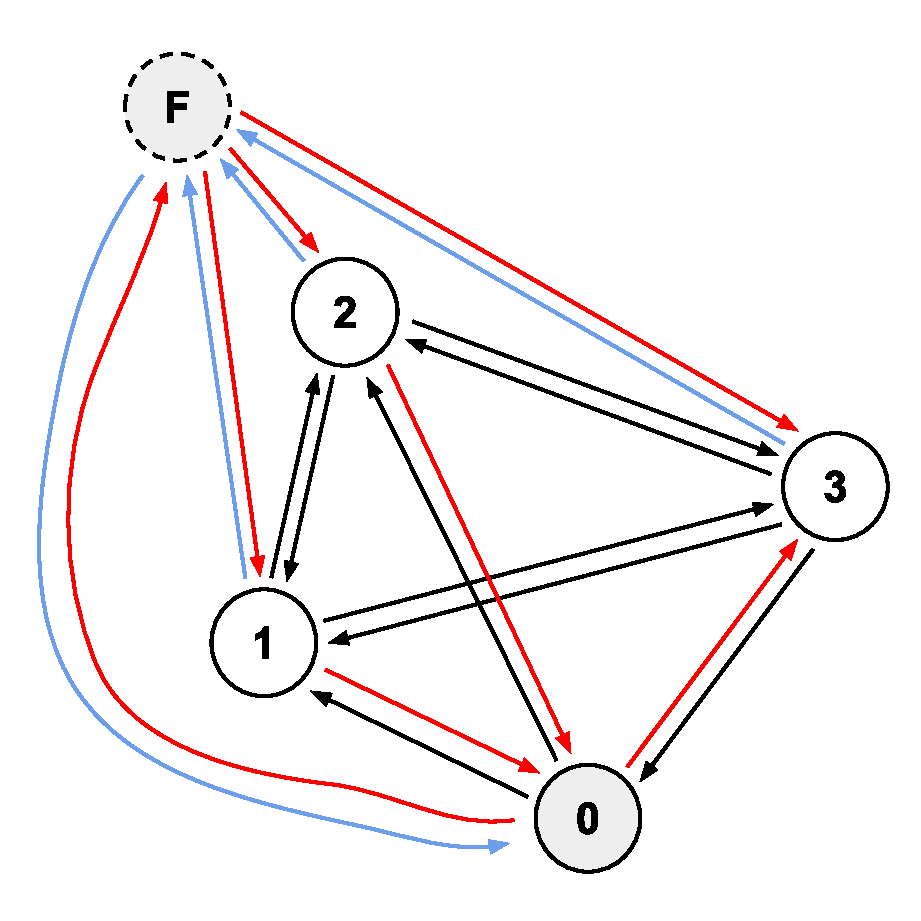
\includegraphics[width=0.4\textwidth]{./fig/photos/TSP.eps}
    \caption{An illustration of the modified distance matrix $\mathbf{D}_{mod}$ for the \ac{TSP} solver, that finds the optimal sequence of waypoints for each \ac{UAV}. 
    The vertex $v_{0}$ is the starting point of the sequence, vertices $\{v_{1}, v_{2}, v_{3}\}$ represent the waypoints to be visited by the \ac{UAV}, $v_{F}$ is an additional dummy virtual vertex. 
    The black edges represent the euclidean distance between corresponding vertices, the value of red edges is set to positive constant $M$, the value of blue edges is set to $0$. }
    \label{fig:tsp}
\end{figure}
%The modified distance matrix $\mathbf{D}_{mod}$ is then passed to the numerical solver.%%}

%%%%%%%%%%%%%%%%%%%%%%%
%%%% PATH PLANNING %%%%
%%%%%%%%%%%%%%%%%%%%%%%
\section{Path planning}% %%{
Once the sequence of waypoints for each \ac{UAV} is determined, the last step is a path planning.
The paths should be collision-free, the minimal distance between each pair of \ac{UAV}s should be at least $\SI{4}\meter$).
The planning method is based on astar planner implemented in the mrs uav system \cite{mrs_system}.
Each \ac{UAV} is assigned a certain priority.
The planning method is described in algorithm \ref{alg:planning}.
The paths are planned sequentially for each drone based on its priority.
Once a path for a drone is generated, the inflated (by the safety distance radius $r = \SI{4}\meter$) points of the path are considered as obstacles for all drones with the lower priority.
If any of the waypoints is not reachable (for example some drone with higher priority planned path in close distance to it), the waypoint is skipped.
The path is then smoothed by the mrs uav system \cite{mrs_system} onboard the drone and executed by the drone's controller.







\begin{algorithm}[!h]
\caption{Multi-path planning}\label{alg:cap}
\begin{algorithmic}

\Function {plan\_paths}{$drones\_waypoints, drones\_poses$}
  \State $planned\_paths \gets \{\}$
  \For {$drone \in drones$} \Comment{iterate over drones based on priority}
    \State $obstacles \gets \{\}$
    \For {$path \in planned\_paths$}
      \State $obstacles \gets obstacles \cup \Call{inflate\_points}{path}$ %\Comment{mark positions around already planned paths as obstacles}
    \EndFor
    \State $path \gets \{\}$
    \State $segment\_start \gets drone\_pose$
    \For {$waypoint \in drone\_waypoints$}

      \If{ $waypoint \in obstacles$}
        \State \textbf{continue}
      \EndIf
      \State $path\_segment \gets \Call{astar\_planner}{start, waypoint, obstacles}$
      \State $segment\_start \gets waypoint$
      \State $path \gets path \cup path\_segment$
    \EndFor
    \State $planned\_paths \gets planned\_paths \cup path$
  \EndFor
  \State \Return $planned\_paths$
\EndFunction


\end{algorithmic}
  \label{alg:planning}
\end{algorithm}% %%}





\mycomment{% %%{
  \subsection{Waypoint generation}
  s a first step, the $\lambda$ matrix (containing the current estimate of sources position) is processed by a local maximum filter. 
  The maximum filter works by sliding a window of a specified size over the $\lambda$.
  The central position of the sliding window is highlighted as local maxima if it is greater than all other values in the sliding window.

  Each waypoint (local maxima) is assigned with a weight $w$.
  The weight is defined as follows:
  \begin{equation}
    w_{j} = \frac{\lambda_{j}}{s_{j_{normalised}}}
  \end{equation},
  where $s_{j_{normalised}} = \frac{s_{j}}{\max_{J}( s_{j})}$ is a sensitivity value for given position $s_{j}$ divided by.
  Such formulation of $w_{j}$ prioritise the points with the highest current estimate of ionizing radiation, that are less explored (have lower sensitivity).

  \begin{algorithm}
  \caption{Planning pipeline}\label{alg:cap}
  \begin{algorithmic}
    \State $POI \gets \Call{get\_points\_of\_interest}$
    \State $POI_{sorted} \gets \Call{filter\_points}{POI}$
    \State $POI_{exploration} \gets \Call{get\_unexplored\_area\_points}$
    
    \State $future\_poses \gets \Call{get\_future\_drone\_poses}$

    \State $W_{exploitation} \gets \Call{clustering}{future\_poses}$
    \State $W_{exploration} \gets \Call{clustering}{future\_poses}$
    
    \State
  \end{algorithmic}
  \end{algorithm}



}% %%}




%% --------------------------------------------------------------
%% |                How to write thesis in LaTeX                |
%% --------------------------------------------------------------


%!TEX root = ../main.tex

\chapter{Results\label{chap:results}}

\section{Monte Carlo simulation}


% Answer: [trim={left bottom right top},clip]
\newpage

\begin{figure}[!htb]% %%{
  \centering
  \subfloat[$p(\mathrm{cone\ detected})$] {
    \centering
    \includegraphics[width=0.5\textwidth,trim={1cm 1cm 2.5cm 1cm},clip]{./fig/photos/monte_carlo_final_prob.eps}
    \label{fig:monte_finalll}
  }
  \subfloat[\ac{pix} sensor geometry.] {
    \centering
    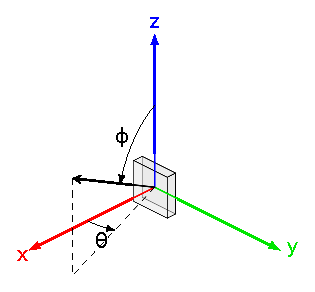
\includegraphics[width=0.5\textwidth]{./fig/photos/axes.eps}
    \label{fig:monte_axes}
  }
  \newline
  \noindent
  \subfloat[$p(\mathrm{reaching\ the\ sensor})$] {
    \includegraphics[width=0.5\textwidth,trim={1cm 1cm 1cm 1cm},clip]{./fig/photos/monte_carlo_total_activity.eps}
    \label{fig:monte_reaching}
  }
  \subfloat[$p(\mathrm{cone\ detected}\ |\ \mathrm{reaching\ the\ sensor})$] {
    \includegraphics[width=0.5\textwidth,trim={1cm 1cm 1cm 1cm},clip]{./fig/photos/monte_carlo_fraction.eps}
    \label{fig:monte_cone_from_hitting}
  }
  \caption{Direction sensitivity of the \ac{pix} sensor (geometry of the sensor depicted in \ref{fig:monte_axes}). 
  Probability that a $\SI{662}{\kilo\electronvolt}$ photon emitted at corresponding position causes a Compton cone is depicted in \ref{fig:monte_finalll}. 
  Probability that particle emitted at given position reaches the detector is depicted in \ref{fig:monte_reaching}. 
  Lastly, probability that a photon (that reached the sensor) causes a Compton cone is illustrated in figure \ref{fig:monte_cone_from_hitting}. }
  \label{fig:monte_clar}
\end{figure}% %%}

\newpage
\section{Real-world (Experiment 1)}% %%{

\begin{figure}[!htb]% %%{
  \centering
  \subfloat[estimate of sources locations $\bm{\lambda}$ (normalized)] {
    \includegraphics[width=0.5\textwidth,trim={0 0.5cm 2cm 1cm},clip]{./fig/photos/auto_lam.eps}
    \label{fig:}
  }
  \subfloat[ground truth positions of sources ($\si{\mega\becquerel}$)] {
    \includegraphics[width=0.5\textwidth,trim={0 0.5cm 2cm 1cm},clip]{./fig/photos/auto_gt.eps}
    \label{fig:}
  }
  \newline
  \noindent 
  \subfloat[back projection (number of Compton cones)] {
    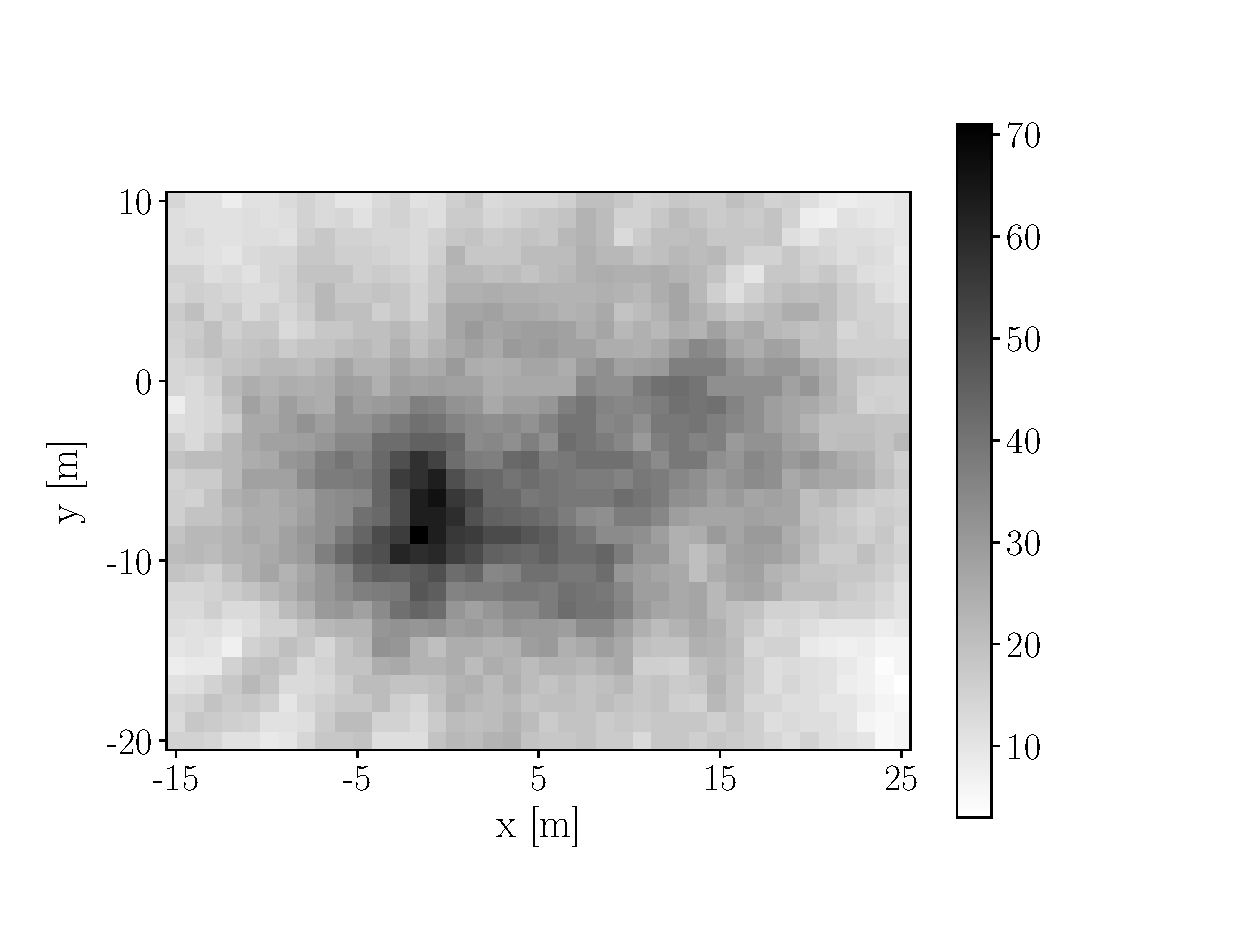
\includegraphics[width=0.5\textwidth,trim={0 0.5cm 2cm 1cm},clip]{./fig/photos/auto_bp.eps}
    \label{fig:}
  }
  \subfloat[sensitivity of detection $\mathbf{s}$] {
    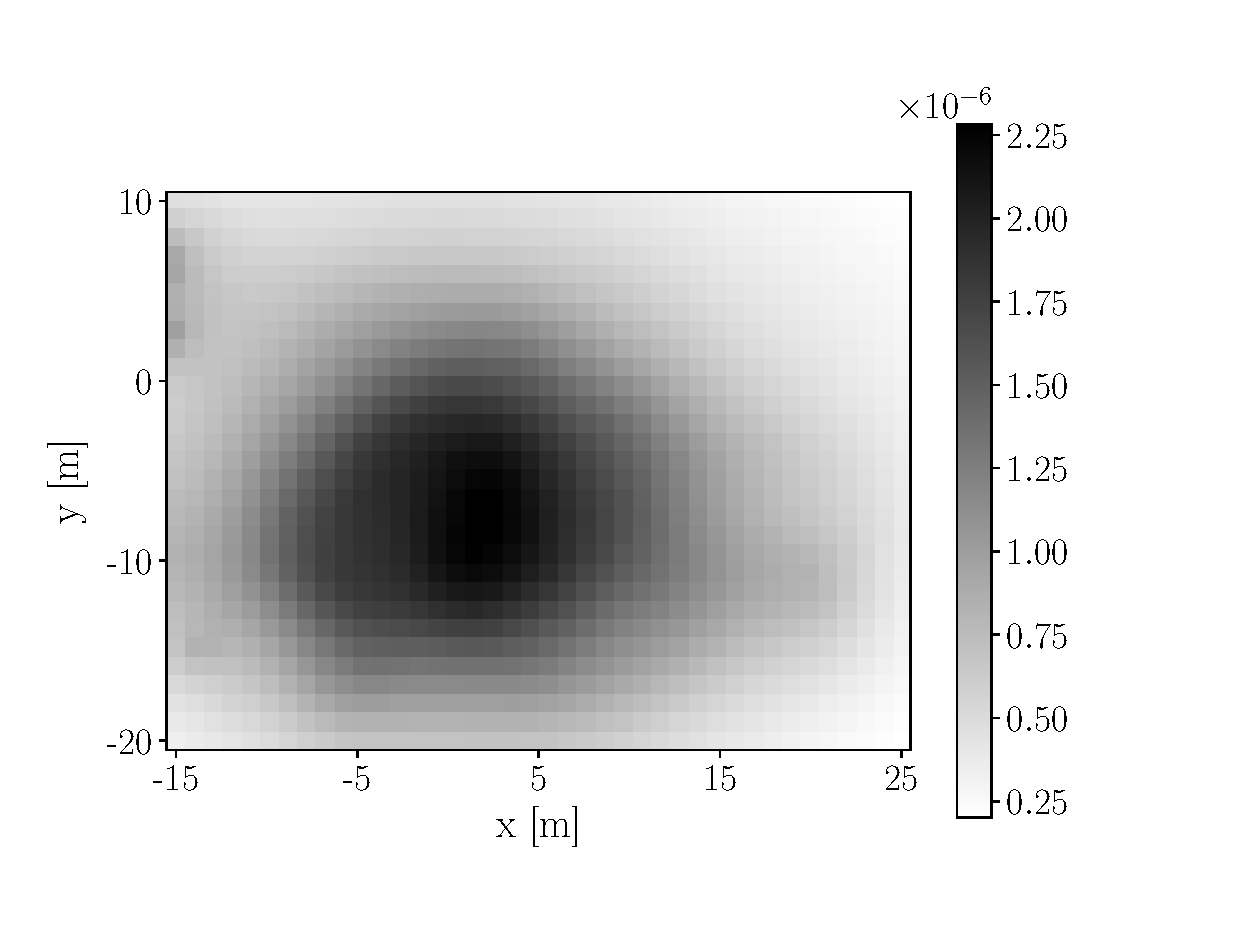
\includegraphics[width=0.5\textwidth,trim={0 0.5cm 2cm 1cm},clip]{./fig/photos/auto_sen.eps}
    \label{fig:}
  }
  \newline
  \noindent 
  \subfloat[] {
    \includegraphics[width=0.5\textwidth,trim={0 0.5cm 2cm 1cm},clip]{./fig/photos/auto_mse_realworld.eps}
    \label{fig:}
  }
  \caption{Results of Monte carlo simulation for cs137.Lorem ipsum  Lorem ipsum Lorem ipsum Lorem ipsum Lorem ipsum Lorem ipsum Lorem ipsum Lorem ipsum Lorem ipsum Lorem ipsum Lorem ipsum Lorem ipsum Lorem ipsum Lorem ipsum Lorem ipsum Lorem ipsum Lorem ipsum Lorem ipsum Lorem ipsum Lorem ipsum Lorem ipsum Lorem ipsum Lorem ipsum Lorem ipsum Lorem ipsum Lorem }
  \label{fig:}
\end{figure}% %%}

setup 
4 drones, 3 seraching, 1 encircling the hypothesis
initial phase: sweeping until 3 cones detected

found the 500 MBq source

To say
x
x
x






% %%}

\newpage
\section{Simulation (experiment 2)}% %%{

\begin{figure}[!htb]
  \centering
  \subfloat[estimate of sources locations $\bm{\lambda}$ (normalized)] {
    \includegraphics[width=0.5\textwidth,trim={0 0.5cm 2cm 1cm},clip]{./fig/photos/auto_simulation_lam.eps}
    \label{fig:}
  }
  \subfloat[ground truth positions of sources ($\si{\mega\becquerel}$)] {
    \includegraphics[width=0.5\textwidth,trim={0 0.5cm 2cm 1cm},clip]{./fig/photos/auto_simulation_gt.eps}
    \label{fig:}
  }
  \newline
  \noindent 
  \subfloat[back projection (number of Compton cones)] {
    \includegraphics[width=0.5\textwidth,trim={0 0.5cm 2cm 1cm},clip]{./fig/photos/auto_simulation_bp.eps}
    \label{fig:}
  }
  \subfloat[sensitivity of detection $\mathbf{s}$] {
    \includegraphics[width=0.5\textwidth,trim={0 0.5cm 2cm 1cm},clip]{./fig/photos/auto_simulation_sen.eps}
    \label{fig:}
  }
  \newline
  \noindent 
  \subfloat[] {
    \includegraphics[width=0.5\textwidth,trim={0 0.5cm 2cm 1cm},clip]{./fig/photos/auto_mse_simulation.eps}
    \label{fig:}
  }
  \caption{Results of Monte carlo simulation for cs137.Lorem ipsum  Lorem ipsum Lorem ipsum Lorem ipsum Lorem ipsum Lorem ipsum Lorem ipsum Lorem ipsum Lorem ipsum Lorem ipsum Lorem ipsum Lorem ipsum Lorem ipsum Lorem ipsum Lorem ipsum Lorem ipsum Lorem ipsum Lorem ipsum Lorem ipsum Lorem ipsum Lorem ipsum Lorem ipsum Lorem ipsum Lorem ipsum Lorem ipsum Lorem }
  \label{fig:}
\end{figure}% %%}

\newpage
\section{Real-world simulation (experiment 3)}% %%{

% Answer: [trim={left bottom right top},clip]
% Ex. 1: trim from left edge

%\includegraphics[width=0.5\textwidth,trim={0 0 2cm 2cm},clip]{./fig/photos/auto_temesvar_drone_paths.eps}


\begin{figure}[ht!]
  \centering
  \subfloat[final estimate of source intensities $\bm{\lambda}$] {
    \includegraphics[width=0.5\textwidth,trim={1cm 0 2.5cm 1cm},clip]{./fig/photos/auto_temesvar_lam.eps}
    \label{fig:}
  }
  \subfloat[ground truth ($\si{MBq}$)] {
    \includegraphics[width=0.5\textwidth,trim={1cm 0 2.5cm 1cm},clip]{./fig/photos/auto_temesvar_gt.eps}
    \label{fig:}
  }
  \newline
  \noindent 
  \subfloat[Sensitivity $\mathbf{s}$ after the initial phase.] {
    \includegraphics[width=0.5\textwidth,trim={1cm 0 2.5cm 1cm},clip]{./fig/photos/auto_temesvar_senzig.eps}
    \label{fig:}
  }
  \subfloat[Sensitivity $\mathbf{s}$ at the end of the experiment.] {
    \includegraphics[width=0.5\textwidth,trim={1cm 0 2.5cm 1cm},clip]{./fig/photos/auto_temesvar_sen.eps}
    \label{fig:}
  }
  \newline
  \noindent 
  \subfloat[Paths of \ac{UAV}s during the search phase (red, green --- exploitation, blue --- exploration)] {
    \includegraphics[width=0.5\textwidth,trim={1cm 0 2.5cm 1cm},clip]{./fig/photos/auto_temesvar_drone_paths.eps}
    \label{fig:}
  }
  \subfloat[Final back-propagation.] {
    \includegraphics[width=0.5\textwidth,trim={1cm 0 2.5cm 1cm},clip]{./fig/photos/auto_temesvar_bp.eps}
    \label{fig:}
  }

  \caption{Results of Monte carlo simulation for cs137}
  \label{fig:}
\end{figure}% %%}

\begin{figure}[!htb]
  \centering
  \subfloat {
    \includegraphics[width=0.7\textwidth]{./fig/photos/experiments.jpg}
  }
  \caption{Field experiments with real hardware.}
  \label{fig:}
\end{figure}


\mycomment{% %%{

\section{Monte carlo simulation results}
In figure \ref{fig:monte_cs_results}, the probability of a Cesium-137 photon generating a Compton cone when emitted from a distance of 1 meter is displayed. 
The sensor's sensitivity is observed to be nearly uniform regardless of the incoming particle's direction. 
This outcome can be explained using Figure \ref{fig:monte_clar}. 
As illustrated in figure \ref{fig:monte_reaching}, particles that approach the sensor from the front side have a greater visible surface area, resulting in a greater likelihood of hitting the sensor. 
Conversely, particles arriving from the side have a longer intersection with the sensor's material, resulting in a greater probability of producing a Compton cone, as shown in figure \ref{fig:monte_cone_from_hitting}. 
Surprisingly, these two effects compensate for each other, resulting in an almost consistent sensitivity of the sensor to particles arriving from various directions.

\begin{figure}[!htb]
  \centering
  \subfloat {
    \includegraphics[width=0.7\textwidth]{./fig/photos/monte_carlo_final_prob.eps}
  }
  \caption{$p(\mathrm{cone\ detected})$ - probability that particle emitted at certain position produces a compton cone.}
  \label{fig:monte_cs_results}
\end{figure}


\section{Evaluation on recorded real-world data}
TODO
\section{Simulations in gazebo}

\section{Real-world experiment with simulated sources}

\subsection{Experimental setup}
The radiation mapping pipeline was tested on a real hardware during the field experiments.
Three \ac{UAV} were used during this experiment.
The real radioactive sources were replaced with simulated ones, the Compton camera simulator \cite{TODO} was running onboard each \ac{UAV}.
All the drones were localized using \ac{gps} in the same coordinate frame and the positions of simulated sources were shared among them.
The size of mapped area was set to $100 \times 100$ m, four simulated sources with activities 500 MBq, 1 GBq, 2 GBq and 2 GBq were placed in the area.
Resolution of the map was $0.5$ m.

\subsection{Results}
\begin{table}[htb]
\begin{center}
  \begin{tabular}{ |c|c|c|c| } 
 \hline
    \multicolumn{2}{|c}{Sources} &  \multicolumn{2}{|c|}{ relative activity } \\
 \hline
    position & activity & ground truth & MLEM estimate\\ 
 \hline
    (10, 20) & 2000 MBq & 1.0  & \textbf{1.0} \\ 
    (20, 20) & 1000 MBq &  0.5 & \textbf{0.49} \\ 
    (80, 80) & 1000 MBq &  0.5 & \textbf{0.52} \\ 
    (75, 75) & 500 MBq &  0.25 & \textbf{0.0} \\ 
 \hline
\end{tabular}
  \caption{Results of the real world experiment with simulated data. Last column presents estimated relative activity at the map positions that correspond to the ground truth position of the given source.}
  \label{tab:temenight_results}
\end{center}
\end{table}

% Answer: [trim={left bottom right top},clip]
% Ex. 1: trim from left edge


\begin{figure}[!htb]
  \centering
  \subfloat {
    \includegraphics[width=0.7\textwidth]{./fig/photos/auto_mse_realworld.eps}
  }
  \caption{$p(\mathrm{cone\ detected})$ - probability that particle emitted at certain position produces a compton cone.}
  \label{fig:monte_cs_results}
\end{figure}


}% %%}

\mycomment{% %%{
    This section describes experiments and evaluation of performance of the proposed method for mapping of ionizing radiation.
    An experiment with real sources of ionizing radiation requires (due to specific safety measures, permission from the state authorities...) coordination with other institutions, such as Czech metrology institute.
    Unfortunately, it was not possible to perform experiment with real sources before the deadline of the thesis due to these organizational reasons.
    However, the method was evaluated on pre-recorded data from real-world experiments as well as using the realistic simulator for compton camera \cite{TODO}.
}% %%}

\mycomment{% %%{




    \section{Pre-recorded data with real radioactive sources}


    \section{Gazebo simulations with the simulated Compton camera}

    \section{Real-world experiment with the simulated Compton camera}



    The approach presented in the previous section was applied on a prerecorded rosbag from a real-world experiment.
    Four \ac{UAV}s were used in this experiment.
    The mapped area was $50 \times 35$ meters with $0.4$ m resolution.
    The experiment took approximately 8 minutes and 250 cones were measured.

    The estimated vector of $\bf{\lambda}$ is presented in figure \ref{fig:D}. 
    The ground truth positions of radioactive sources with their strength can be seen on figure \ref{fig:C}.
    The sensitivity vector $\mathbf{s}$ and the matrix $\mathbf{T}$ summed over all measurements (which serves as simple projection of the cones to the map) are presented in figures \ref{fig:E} and \ref{fig:F}.
    \begin{figure}[!h]
      \centering
      \subfloat[True positions of sources (MBq)] {
        \includegraphics[width=0.5\textwidth]{./fig/photos/temenight_ground_truth.eps}
        \label{fig:C}
      }
      \subfloat[MLEM estimate after 10 iterations] {
        \includegraphics[width=0.5\textwidth]{./fig/photos/temenight_lambdas.eps}
        \label{fig:D}
      }
      \label{fig:A}
      \caption{Comparison of \ac{MLEM} algorithm estimate and the ground truth.}
    \end{figure}

    \begin{figure}[!htb]
      \centering
      \subfloat[System matrix $\mathbf{T}$ summed over $\forall i$] {
        \includegraphics[width=0.5\textwidth]{./fig/photos/temenight_back_projection.eps}
        \label{fig:E}
      }
      \subfloat[Sensitivity vector $\mathbf{s}$] {
        \includegraphics[width=0.5\textwidth]{./fig/photos/temenight_sensitivity.eps}
        \label{fig:F}
      }
      \label{fig:B}
      \caption{System matrix and sensitivity vector estimated during the experiment}
    \end{figure}

    \section{Discussion}
    We can see that the algorithm precisely detected the 500 MBq source. Two smallest source were not recognised, probably due to low number of cones measured.
    The 1900 MBg source was partially detected. 
    In is important to note that the drones were flying mostly around the 500 MBg source and most of the measured cones originated from that source, as we can see in the sensitivity vector and system matrix.
    This approach seems to be beneficial compared to naive back-projection of the cones to the map (without weighting with the sensitivity), since it can "see" the 1900 MBq source despite the fact that only few cones originated there.


}% %%}

%% --------------------------------------------------------------
%% |                         Conclusion                         |
%% --------------------------------------------------------------

%!TEX root = ../main.tex

\chapter{Conclusion\label{chap:conclusion}}
The goal of this thesis was to research, design, and implement an algorithm and software method for collaborative sensor fusion of
measured ionizing radiation data from a group of \ac{UAV}s.
The presented solution based on the \ac{MLEM} algorithm is able to localize multiple sources of ionizing radiation based on data acquired by a group of drones equipped with a miniature Compton camera. All the subtasks in the thesis assignment were fulfilled:
\begin{itemize}
  \item The author of the thesis familiarized himself with the MRS UAV System and the principles of the Compton camera detector. 
The use of MRS UAV System was demonstrated during simulated and real-world experiments described in Chapter \ref{chap:results}. 
An overview of the principles of the Compton camera is presented in Chapter \ref{chap:preliminaries}.
  \item A method for the localization of multiple sources of ionizing radiation using the Compton camera measurements was implemented. 
The online estimation method is based on the \ac{MLEM} algorithm, which was adapted to the proposed application.
The directional sensitivity of the \ac{pix} sensor was studied using Monte Carlo simulation.
    The proposed method takes into account the sensitivity of detection (how likely a potential source at a certain position has been detected by the \ac{UAV}s during the flight), which improves the quality of estimate in scenarios with multiple sources of radiation with different emission activity.
The proposed localization method is presented in Chapter \ref{chap:methods_estimation}.
  \item The proposed active search strategy for a small group of \ac{UAV} is presented in Chapter \ref{chap:methods_robotics}.
    The centralized search strategy takes the current estimate of radioactive sources as an input and generates waypoints for the \ac{UAV}s in order to acquire more measurements and explore less explored parts of the area.         
    The generated waypoints are assigned to the individual drones, and a non-colliding path connecting the waypoints is computed for each drone.
  \item The proposed estimation method and the search strategy were evaluated on recorded real-world data and in simulation, as presented in Chapter \ref{chap:results}.
    %Experiments with recorded real data showed that the proposed method is able
    The functionality of the whole system was also demonstrated during outdoor experiments with real hardware and simulated sources of radiation 
    (in addition to the scope of the thesis assignment). 
\end{itemize}

\section{Discussion}
In summary, the proposed method for radiation mapping, in combination with the active search strategy, proved to be applicable for the task of localization of multiple sources of ionizing radiation.
Let us summarize the properties of the proposed solution and its limitations.

Many limiting factors originate in the nature of the \ac{pix} sensor, Compton measurements and properties of ionizing radiation.
The biggest issue is the limited number of data that is given by the relatively low sensitivity of the \ac{pix} sensor.
The limited sensitivity is given by the fact that the sensor is very small and that only less than $\approx 1\%$ of gamma photons (based on the Monte Carlo simulation) reaching the semiconductor \ac{CdTe} detection block cause the Compton event.
Therefore less active sources (with emission activity of hundreds of $\si{\mega\becquerel}$ and less) might not be easily detected by the proposed multi-robot system (more precisely, their detection requires longer time spend in the vicinity of the source).
The working principle of the single-layer Compton camera (where the corresponding interactions are paired together based on their times of arrival) 
also limits the sensitivity of the \ac{pix} sensor (working as the Compton camera) in scenarios with high emission activity of radioactive sources.
If the number of interactions inside the \ac{CdTe} semiconductor block is too high, the sensor can no longer correctly deduce which interactions should be paired together, and the number of outliers increases (this is more a speculation based on the author's understanding of the sensors working principle, since the recorded data did not contain scenarios of sources with activity higher than $\SI{2}{\giga\becquerel}$ and the simulator cannot properly model this effect).
The effect of the very active sources on the detection capability of the \ac{pix} sensor needs to be investigated.
However, we can conclude that the proposed method is suitable for the detection of sources with mid-level emission activity and cannot detect sources with very low or high activity).

Another limitation is that the output of the proposed \ac{MLEM} method does not provide any absolute information about the emission activity of the source.
Although the optimized hidden parameters $\bm{\lambda}$ have meaning of expected emission rate, 
it turned out that the number of measured Compton cones ($\approx 10^{2}-10^{3}$) during recorded real-world experiments was not sufficient to accurately model the absolute emission activity of the source
and the output of the \ac{MLEM} method can serve only as information about the relative emission activity of the sources present in the area.
Another problem is that the \ac{MLEM} method does not provide any guarantees on the quality of the estimate.
Therefore the method can be used for fast and inaccurate detection of possible hot spots in unknown areas (and the estimated source needs to be further verified by other types of sensors that can accurately estimate the activity of the detected source).

Unlike the solution described in \cite{baca2021gamma} for single-source localization using \ac{LKF}, the proposed method can't localize the moving source of ionizing radiation.
The solution proposed in \cite{baca2021gamma} based on \ac{LKF} is better suited for scenarios with single source and very low number of measurements ($\approx 10$).
The maximum likelihood method generally requires more data to produce accurate estimates of the underlying probability distribution, which is partially compensated by the active search strategy.

\section{Future work}
The experiments with recorded real-world data showed that the real measurements acquired by the \ac{pix} sensor contain many outliers and noise in the measurements that significantly affected the quality of \ac{MLEM} reconstruction.
Experiments in simulation (with simulated noise) showed that the proposed active search strategy is able to overcome the noise in measurements by controlling the drones to get more data.
However, the combination of the proposed search strategy and the \ac{MLEM} estimation method could not be tested with real sources of ionizing radiation (due to organizational reasons).
Future testing with real Cesium-137 sources is therefore needed for accurate evaluation.
Further investigation of parameters influencing the quality of reconstruction also presents a task for future.

Another possible improvement of the proposed method is optimal planning and task allocation during the search strategy.
More advanced state-of-the-art methods can be applied, such as solving multi-robot orienteering problem when planning the future movement of the drones, better task allocation methods or coverage path planning for the exploration.
In general, the search strategy can be optimized by applying some global planning methods.

The proposed localization method was developed for 2D radiation mapping in an outdoor open area.
A possible future extension is to fuse the Compton measurements with a 3D map of the environment (computed by some \ac{SLAM} method based on \ac{LiDAR} data).
The set of obstacles generated by the \ac{SLAM} method can be used as a set of possible source locations in the \ac{MLEM} algorithm.
This would open the possibility of monitoring radiation even in areas with obstacles or in the indoor environment.
Fusion of the direction-based Compton camera sensor with some intensity based detectors might help to estimate not only the realitve, but also absolute emission activity of the source. 


%The stochastic nature of radioactive decay and limited sensing range of detectors (caused by properties of radiation spread in the environment) implies strong dependency between the drones' trajectories and quality of measurements.

%Testingi
%The proposed active search strategy helps to improve the quality of \ac{MLEM} estimate by controlling the drones based on the current estimate.
%However, the combination of the proposed radiation mapping method and search strategy was not tested on real radiation sources.



%The experiments showed that the quality of sources localization strongly depends on the measured data (given the stochastic nature of radioactive sources and limited sensing range of detectors caused by properties of ionizing radiation).

%therefore an active search strategy significantly 


\mycomment{
In this thesis, a method for collaborative sensor fusion of measured ionizing radiation data from a group of unmanned aerial vehicle was presented.


\alertwarning{Under construction}
The solution for the localization of multiple sources of ionizing radiation was presented.
The sensory fusion algorithm is based on the maximum likelihood expectation maximization approach.
To summarize, a small group of \ac{UAV}s equipped with Compton camera sensors are capable of detecting strong sources of ionizing radiation.

\section{Future work}
There are multiple possible improvements.
First of all, a more accurate model for the sensitivity of the Minipix3 sensor (with respect to the direction of incoming gamma particles) should be introduced.
One possible way might be a Monte Carlo simulation.
It should improve the precision of localization.
Secondly, the localization method might be extended into 3D.
An octomap obtained by an onboard lidar sensor might serve as a model of the terrain surface and possible source locations.
Thirdly, some kind of dosimetric data from the sensor might be used to estimate the "strength" of the source and shorten the time needed for localization since the number of particles causing the Compton effect in the Compton camera is relatively small.
Lastly, an active search method should be introduced to shorten the time of localization and control the group of \ac{UAV}s in an optimal way.

to say
it worked
method for mapping of multiple sources was introduced



possible extensions
3D map made with lidar data
%more accurate simulator

%needs testing in real life


TODO
%further testing
%validation in reality
}

%\input{src/how_to_write_thesis.tex}

%% --------------------------------------------------------------
%% |                         References                         |
%% --------------------------------------------------------------

\chapter{References}

\printbibliography[heading=none,title={}]

%% --------------------------------------------------------------
%% |                         Appendices                         |
%% --------------------------------------------------------------

\appendix
\renewcommand\chaptername{Appendix}

\renewcommand{\thechapter}{A}
\renewcommand\chaptername{Appendix A}

\chapter{Appendix A}

\end{document}
